\documentclass[11pt,a4paper]{article}

% ── Core packages ─────────────────────────────────────────────────────────────
\usepackage[utf8]{inputenc}
\usepackage[T1]{fontenc}
\usepackage{microtype}
\usepackage[margin=1in]{geometry}
\usepackage{amsmath,amssymb,amsfonts,amsthm}
\usepackage{graphicx}
\graphicspath{{figures/}}
\usepackage{booktabs}
\usepackage{multirow}
\usepackage{subcaption}
\usepackage{float}
\usepackage{xcolor}
\usepackage{algorithm}
\usepackage{algpseudocode}
\usepackage[round,sort]{natbib}
\usepackage{hyperref}
\usepackage{url}
\usepackage{enumitem}
\usepackage{tabularx}
\usepackage{array}
\usepackage{setspace}
\usepackage{tikz}
\usetikzlibrary{shapes.geometric,arrows,positioning,calc}

% ── Hyperref configuration ────────────────────────────────────────────────────
\hypersetup{
    colorlinks = true,
    linkcolor  = blue!70!black,
    citecolor  = green!50!black,
    urlcolor   = blue!80!black,
    pdftitle   = {Estimating Routing Importance in Transformer Attention Graphs},
    pdfauthor  = {Amit Kumar}
}

% ── Custom maths commands ─────────────────────────────────────────────────────
\newcommand{\R}{\mathbb{R}}
\newcommand{\E}{\mathbb{E}}
\newcommand{\pr}{\text{PR}}
\newcommand{\rie}{\text{RIE}}

\theoremstyle{definition}
\newtheorem{definition}{Definition}[section]
\theoremstyle{plain}
\newtheorem{proposition}{Proposition}[section]

% ── Title block ───────────────────────────────────────────────────────────────
\title{%
    \LARGE\textbf{Estimating Routing Importance in Transformer Attention Graphs}%
}

\author{%
    Amit Kumar\\[2pt]
    \small\textit{Independent Researcher}\\
    \small\texttt{[contact email]}%
}

\date{\today}

% ═════════════════════════════════════════════════════════════════════════════
\begin{document}

\maketitle
\thispagestyle{empty}

% ── Abstract ─────────────────────────────────────────────────────────────────
\begin{abstract}
\noindent
Understanding how information is routed through transformer attention heads is a central challenge in mechanistic interpretability. While existing approaches primarily focus on identifying discrete circuit subgraphs, we investigate whether attention-head necessity can be explained by structural properties of a global routing network. We estimate a directed routing dependency graph over attention heads using causal interventions and derive a family of Routing Importance Estimators ($\rie$) based on node centralities. Through OLS regressions across multiple transformer families (GPT-2, OPT, and Pythia), we demonstrate that these structural routing descriptors explain a substantial fraction of the observed variance in experimentally measured causal head damage (up to $R^2 = 0.802$ on Pythia-160m). Under $F$-testing, these estimators retain highly significant explanatory power beyond simple architectural priors such as layer depth ($p < 10^{-5}$), showing massive effect sizes (up to Cohen's $f^2 = 4.56$ on Pythia-160m). Random shuffling of the head-descriptor correspondence collapses the explained variance to under 1.3\%, confirming that the predictive performance is driven strictly by the underlying network topology. Finally, we instantiate the practical utility of these estimators through FLOOD, a routing-aware pruning algorithm that preserves language modeling perplexity up to $31\times$ better than magnitude-based baselines while maintaining the topological properties of the underlying network.
\end{abstract}

\newpage
\setcounter{page}{1}
\tableofcontents
\vspace{2em}

% ═════════════════════════════════════════════════════════════════════════════
\section{Introduction}
\label{sec:intro}

Mechanistic interpretability seeks to demystify the internal computations of transformer architectures by identifying discrete circuits---subgraphs of attention heads and MLP layers that perform specialized sub-tasks \citep{elhage2021mathematical, olsson2022induction}. While these circuit-level descriptions provide valuable local explanations, they typically treat representational routing as isolated pathways, making it difficult to analyze the network's global structural organization.

In this work, we propose a shift in perspective. Rather than focusing solely on localized sub-circuits, we study the global topological structure of information flow. We establish the following central claim:
\begin{quote}
\itshape
Routing descriptors estimated from causal dependency graphs provide statistically significant explanatory power for experimentally measured attention-head importance beyond simple architectural priors such as layer depth.
\end{quote}

\paragraph{Contributions.}
Specifically, our primary contributions are:
\begin{enumerate}
    \item \textbf{Causal Routing Dependency Graph Estimation:} We propose a methodology to estimate directed routing dependency graphs over attention heads via causal perturbation interventions, characterizing the flow of representations without circuit-level assumptions.
    \item \textbf{Routing Importance Estimator (RIE) Family:} We define a parameterized family of structural graph-centrality descriptors (Broadcast, Receiver, Injector, Betweenness centralities) to represent head routing roles.
    \item \textbf{Statistical Validation centerpiece:} We validate the causal relevance of these descriptors using multiple linear regressions, proving they explain up to 80.2\% of perplexity damage variance, significantly outperform layer-depth controls ($p < 10^{-5}$, with effect sizes up to Cohen's $f^2 = 4.56$), and collapse under randomized shuffle controls ($\le 1.3\%$). We also demonstrate zero-shot out-of-distribution transfer to held-out architectures ($\rho = 0.469$, $p < 0.001$).
    \item \textbf{Topological Downstream Application:} We instantiate the practical utility of RIE via FLOOD, a routing-aware structured attention-head pruning algorithm. FLOOD preserves language modeling perplexity on WikiText-2 up to $31\times$ better than magnitude pruning and maintains the topological backbone of the representations.
\end{enumerate}

To guide the reader, a conceptual overview of our pipeline is illustrated in Figure~\ref{fig:pipeline}. Table~\ref{tab:notation} summarizes the key symbols and notations used throughout the paper.

\begin{figure}[t]
\centering
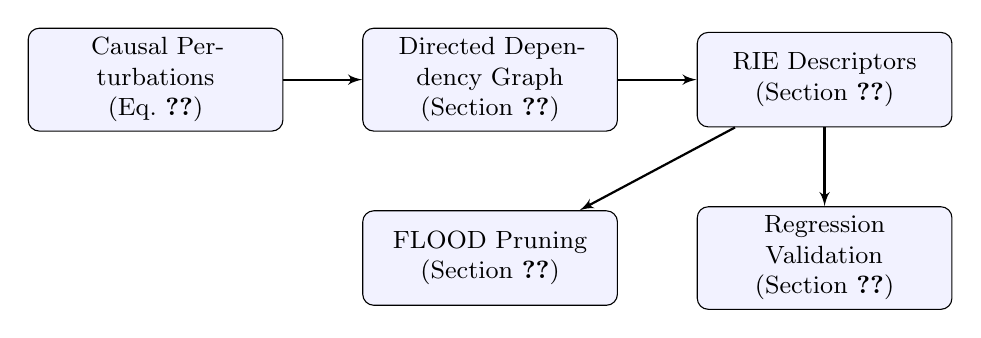
\begin{tikzpicture}[node distance=1.5cm, auto,
    block/.style={rectangle, draw, fill=blue!5, text width=3.0cm, text centered, rounded corners, minimum height=1.2cm, font=\small},
    line/.style={draw, -latex', thick}]
    
    \node [block] (perturb) {Causal Perturbations\\(Eq.~\ref{eq:dependency})};
    \node [block, right=1.0cm of perturb] (graph) {Directed Dependency Graph\\(Section~\ref{sec:discovery})};
    \node [block, right=1.0cm of graph] (rie) {RIE Descriptors\\(Section~\ref{sec:rie})};
    
    \draw [line] (perturb) -- (graph);
    \draw [line] (graph) -- (rie);
    
    \node [block, below=1.0cm of rie] (validation) {Regression Validation\\(Section~\ref{sec:validation})};
    \node [block, left=1.0cm of validation] (pruning) {FLOOD Pruning\\(Section~\ref{sec:application})};
    
    \draw [line] (rie) -- (validation);
    \draw [line] (rie) -- (pruning);
\end{tikzpicture}
\caption{Conceptual pipeline of our research program: from causal interventions to global graph extraction, RIE structural centrality estimation, validation via causal damage regressions, and downstream application via FLOOD pruning.}
\label{fig:pipeline}
\end{figure}

\begin{table}[h]
\centering
\caption{Table of notation and key mathematical symbols.}
\label{tab:notation}
\begin{tabular}{ll}
\toprule
\textbf{Symbol} & \textbf{Meaning} \\
\midrule
$D$ & Dependency matrix representing directed attention head interactions \\
$G$ & Routing dependency graph \\
$\lambda_2$ & Algebraic connectivity (Fiedler value of the graph Laplacian) \\
$Q$ & Graph modularity measuring functional cluster isolation \\
$RIE_\theta$ & Routing Importance Estimator family parameterized by $\theta$ \\
$f_{\text{bcast}}$ & Broadcast Centrality (source-like routing descriptor) \\
$f_{\text{recv}}$ & Receiver Centrality (sink-like routing descriptor) \\
$f_{\text{inj}}$ & Injector Centrality (local feedforward routing descriptor) \\
$f_{\text{bet}}$ & Betweenness Centrality (bottleneck-like routing descriptor) \\
\bottomrule
\end{tabular}
\end{table}

% ═════════════════════════════════════════════════════════════════════════════
\section{Related Work}
\label{sec:related}

\subsection{Structured Pruning of Transformers}
Structured pruning removes entire attention heads or MLP dimensions to improve inference throughput \citep{han2015learning, frankle2019lottery}. Modern methods like SparseGPT \citep{frantar2023sparsegpt} and Wanda \citep{sun2024wanda} perform structured compression on massive models using weight-activation statistics, while LLM-Pruner \citep{ma2023llmpruner} leverages gradient information. However, existing structured pruning methods estimate head necessity from local weight/activation magnitudes or gradients in isolation; in contrast, this work studies routing descriptors derived from a global dependency graph and evaluates whether those descriptors explain experimentally measured causal damage.

\subsection{Attention Head Importance Estimation}
Pruning and interpretation pipelines rely heavily on head importance estimation. \citet{michel2019sixteen} and \citet{voita2019analyzing} demonstrated that a large fraction of self-attention heads can be ablated without significant performance degradation. Common importance estimation strategies employ first-order Taylor expansions over gradients \citep{molchanov2017taylor} or activation magnitudes. However, traditional importance metrics are local and do not capture the downstream relational structure of attention flow; our graph-theoretic estimators model the network-wide dependency cascades to explain causal head necessity.

\subsection{Mechanistic Interpretability and Circuit Discovery}
Mechanistic interpretability aims to reverse-engineer neural representations into discrete computational graphs \citep{elhage2021mathematical}. Key achievements include identifying induction circuits \citep{olsson2022induction} and automated circuit discovery frameworks like ACDC \citep{conmy2023acdc} or causal abstraction \citep{geiger2024causal}. While circuits focus on discrete, localized, task-specific subgraphs, we characterize the global topology of representational routing and show it explains causal head necessity.

\subsection{Graph Representations of Neural Networks}
Graph-theoretic analyses are widely used to study neural network representations and topology. Prior work evaluates network modularity and centrality metrics to characterize model scaling and representation alignment \citep{clark2019bertlook, goldblum2024battle}. However, existing graph models of neural network representations are typically observational (relying on correlation matrices) or post-hoc; we construct causal dependency graphs using systematic interventions to analyze routing importance.

\subsection{Causal Intervention Analysis}
Causal intervention analysis patches or ablates activations to locate critical components. Frameworks like causal mediation analysis \citep{meng2022rome} systematically perturb internal representations to map factual associations and localized causal effects. While activation patching is typically used to locate single task-specific circuits, we apply it globally and exhaustively across the model to estimate a directed flow network over all heads.

% ═════════════════════════════════════════════════════════════════════════════
\section{Discovery: Estimating the Routing Graph}
\label{sec:discovery}

To characterize representational routing without imposing structural circuit assumptions, we estimate a directed routing dependency graph over attention heads using causal perturbation interventions.

\subsection{Causal Dependency Extraction}
Let $M$ be a transformer with $L$ layers and $H$ attention heads per layer, yielding $N = L \times H$ total heads. Let $h_v(x) \in \mathbb{R}^{T \times d_h}$ denote the activation representation of head $v$ at layer $l_v > l_u$ for an input sequence $x$ of length $T$. Let $h_v^{(\backslash u)}(x)$ denote the activations of head $v$ when source head $u$ (at layer $l_u$) is ablated by masking its output projection weights. 

We define the directed dependency weight $D(u, v)$ as the average fractional change in the L2 norm of the activations across sequence positions:
\begin{equation}
    D(u, v) \;=\; \E_{x \sim \mathcal{P}} \left[ \frac{1}{T} \sum_{t=1}^T \frac{\|h_{v, t}(x) - h_{v, t}^{(\backslash u)}(x)\|_2}{\|h_{v, t}(x)\|_2 + \epsilon} \right]
    \label{eq:dependency}
\end{equation}
where $\epsilon = 10^{-8}$ is a numerical stabilizer. For any head pair where $l_v \le l_u$, we set $D(u, v) = 0$ by construction, ensuring a layered directed graph.

\subsection{Global Graph Metrics}
We analyze the global topological structure of the estimated routing graph using two key metrics from network science:
\begin{itemize}
    \item \textbf{Algebraic Connectivity (Fiedler Value $\lambda_2$):} The second smallest eigenvalue of the graph Laplacian, which measures the routing connectivity strength and pathway redundancy \citep{fiedler1973algebraic}.
    \item \textbf{Graph Modularity ($Q$):} Measures the strength of the division of the network into modular, isolated functional clusters \citep{newman2006modularity}.
\end{itemize}

Figure~\ref{fig:dep_network} shows an example of the estimated routing dependency network for GPT-2 Small, displaying the layered layout. Figure~\ref{fig:spectral} presents the spectral Laplacian analysis. Table~\ref{tab:graph_stats} compiles these global topological properties across four evaluated models.

\begin{figure}[t]
\centering
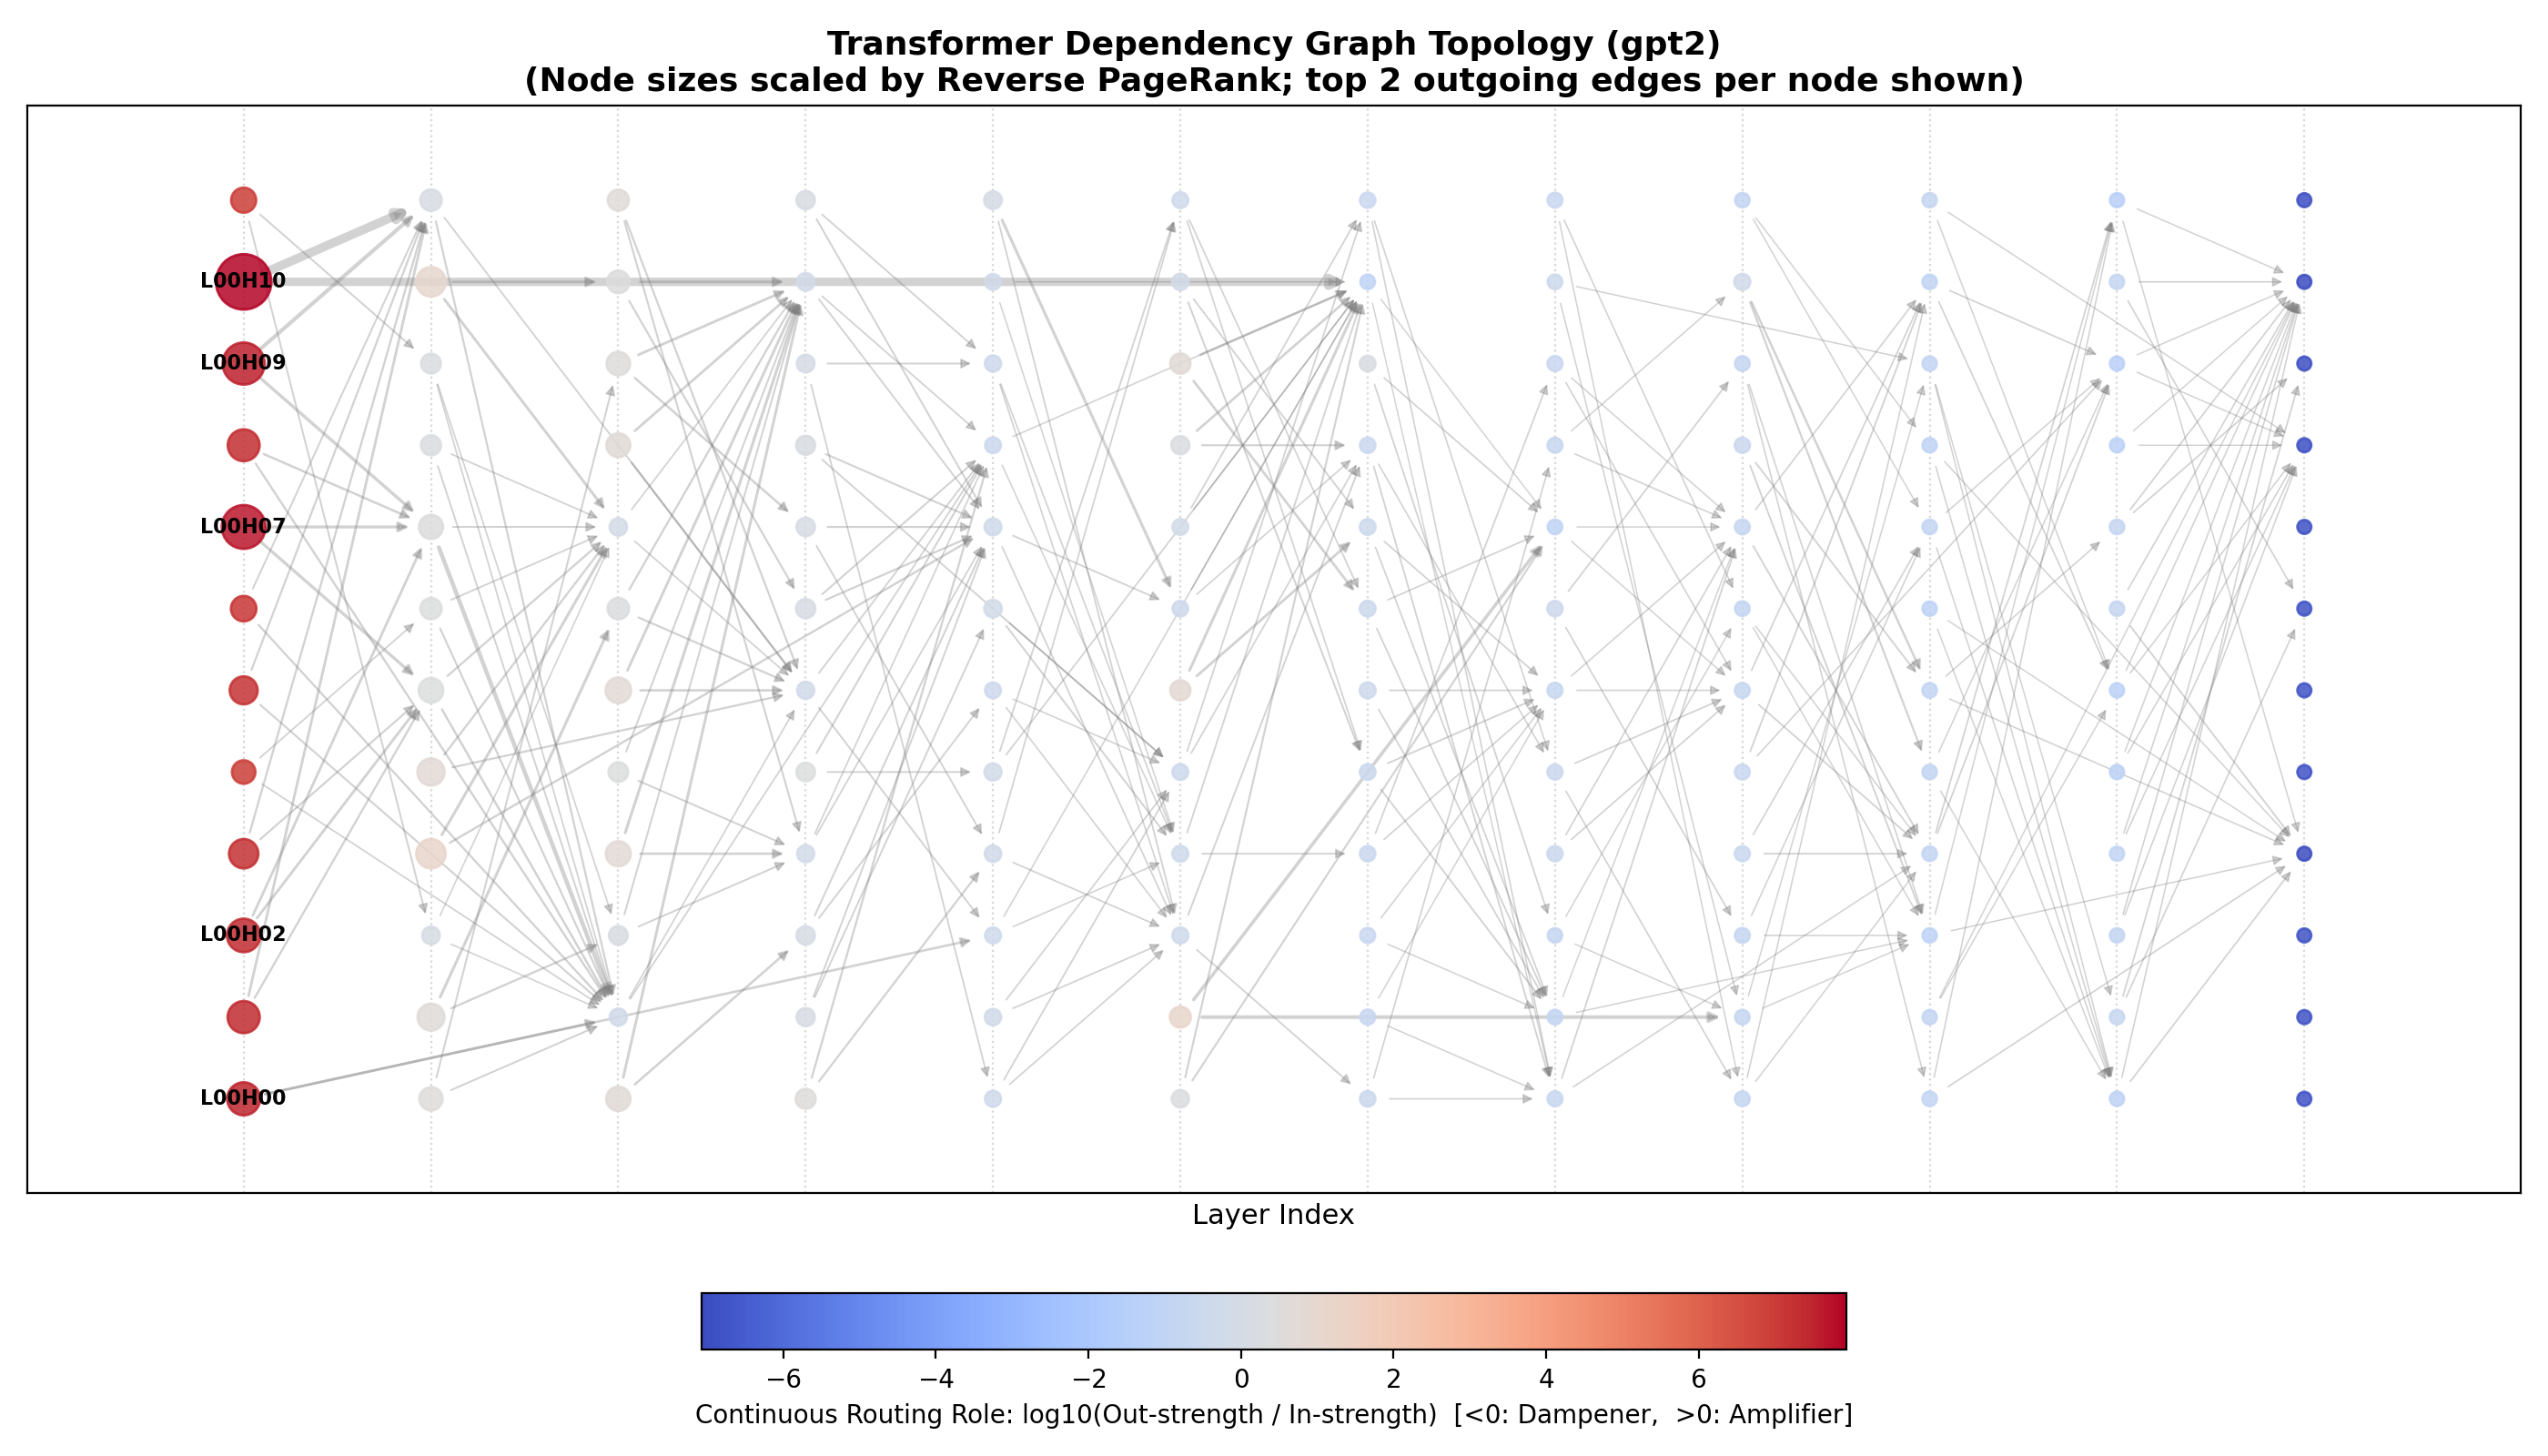
\includegraphics[width=0.7\textwidth]{gpt2_dependency_network_grouped.png}
\caption{Directed routing dependency network $G$ estimated for GPT-2 Small, grouped by layers. The edge weights represent causal dependency strengths $D(u,v)$ between attention heads.}
\label{fig:dep_network}
\end{figure}

\begin{figure}[t]
\centering
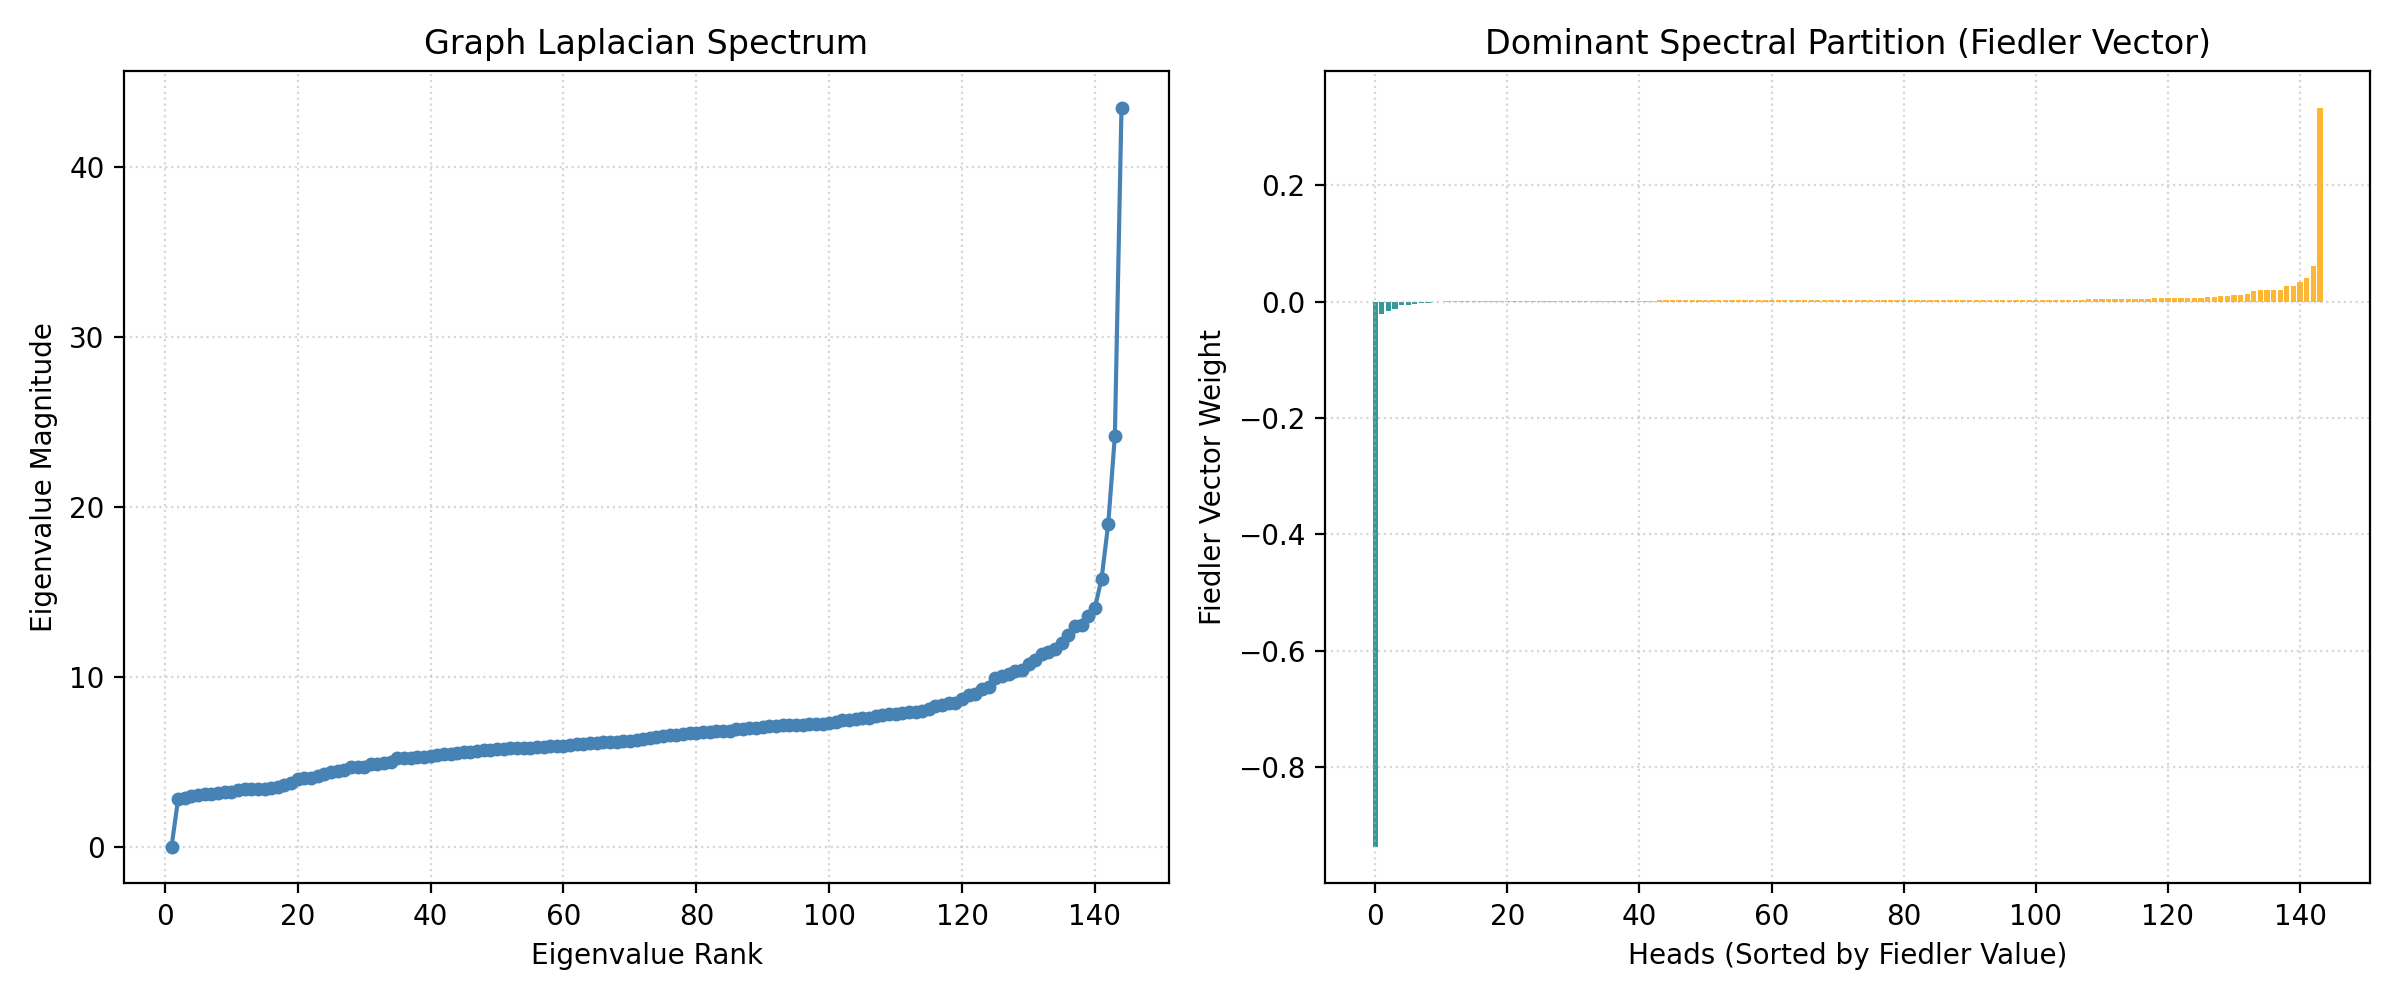
\includegraphics[width=0.7\textwidth]{gpt2_spectral_laplacian.png}
\caption{Spectral Laplacian analysis of the GPT-2 Small routing graph. The eigenvalues are sorted, with the second eigenvalue denoting the Fiedler value $\lambda_2$, measuring graph connectivity.}
\label{fig:spectral}
\end{figure}

\begin{table}[h]
\centering
\caption{Global topological graph statistics and best routing descriptors across models.}
\label{tab:graph_stats}
\begin{tabular}{lcccc}
\toprule
\textbf{Model} & \textbf{Total Heads ($N$)} & \textbf{Algebraic Connectivity ($\lambda_2$)} & \textbf{Graph Modularity ($Q$)} & \textbf{Dominant Descriptor} \\
\midrule
\textbf{OPT-125m} & 144 & 5.6392 & 0.0609 & \textbf{Bridge-Only} \\
\textbf{Pythia-160m} & 144 & 4.6339 & 0.0920 & \textbf{Broadcast-Only} \\
\textbf{GPT-2 Small} & 144 & 2.6931 & 0.1730 & \textbf{Broadcast-Only} \\
\textbf{Pythia-70m} & 48 & 1.7978 & 0.2201 & \textbf{Mixed} \\
\bottomrule
\end{tabular}
\end{table}

\subsection{Observations on Graph Properties and Hypotheses}
We observe a clear empirical relationship between the global graph topology and descriptor dominance:
\begin{itemize}
    \item \textbf{Cohesive Topologies (Low Modularity, High Connectivity):} In models like OPT-125m and Pythia-160m, specific individual descriptors exhibit clear dominance patterns (e.g., Bridge-Only or Broadcast-Only). Across the evaluated models, higher $\lambda_2$ was associated with greater descriptor dominance.
    \item \textbf{Clustered Topologies (High Modularity, Low Connectivity):} In highly modular, loosely connected networks (e.g., Pythia-70m), individual descriptors in isolation fail. The graph is fragmented into isolated clusters, requiring composite or mixed signals to capture functional necessity.
\end{itemize}
We hypothesize that routing connectivity and path redundancy control the extent to which information routing is concentrated in single bottleneck nodes versus distributed across parallel modules.

% ═════════════════════════════════════════════════════════════════════════════
\section{Methodology: Routing Importance Estimators (RIE)}
\label{sec:rie}

We define the Routing Importance Estimator ($\rie$) not as a single handcrafted equation, but as a family of estimators parameterized by a set of weighting coefficients $\theta = \{\alpha_1, \alpha_2, \alpha_3, \alpha_4\}$:
\begin{equation}
    RIE_{\theta}(u) \;=\; \alpha_1 f_{\text{bcast}}(u) + \alpha_2 f_{\text{recv}}(u) + \alpha_3 f_{\text{inj}}(u) + \alpha_4 f_{\text{bet}}(u)
    \label{eq:rie_family}
\end{equation}
where $f_i(u)$ represent standardized node centralities computed from the estimated routing graph $G$:
\begin{enumerate}
    \item \textbf{Broadcast Centrality ($f_{\text{bcast}}$):} Measures the extent to which a head acts as a global information source. Computed via PageRank on the transpose dependency matrix (reverse PageRank) \citep{page1999pagerank}:
    \begin{equation}
        f_{\text{bcast}}(u) \;=\; d \sum_{v \ne u} \frac{D(v, u)}{\text{out-degree}(v)} f_{\text{bcast}}(v) + \frac{1-d}{N}
    \end{equation}
    \item \textbf{Receiver Centrality ($f_{\text{recv}}$):} Measures the extent to which a head acts as a global information sink. Computed via forward PageRank:
    \begin{equation}
        f_{\text{recv}}(u) \;=\; d \sum_{v \ne u} \frac{D(u, v)}{\text{in-degree}(v)} f_{\text{recv}}(v) + \frac{1-d}{N}
    \end{equation}
    \item \textbf{Injector Centrality ($f_{\text{inj}}$):} Measures local feedforward influence to the immediate next layer, representing direct downstream injection:
    \begin{equation}
        f_{\text{inj}}(u) \;=\; \sum_{v \in \text{layer } l_u+1} D(u, v)
    \end{equation}
    \item \textbf{Betweenness Centrality ($f_{\text{bet}}$):} Measures local bottleneck intensity by calculating the proportion of shortest routing paths passing through a head \citep{freeman1977betweenness}.
\end{enumerate}

To instantiate this practically, we introduce the FLOOD algorithm. Pseudocode for RIE scoring and FLOOD pruning is detailed in Algorithm~\ref{alg:flood}.

\begin{algorithm}[H]
\caption{RIE Scoring and FLOOD Attention Head Pruning}
\label{alg:flood}
\begin{algorithmic}[1]
\State \textbf{Input:} Model $M$ with attention heads $\{1, \dots, N\}$, calibration prompts $\mathcal{P}$, pruning ratio $K$.
\State \textbf{Step 1: Dependency Matrix Extraction}
\For{each pair of heads $u, v$ where $l_v > l_u$}
    \State Measure activation shift $D(u, v)$ under ablation of $u$ using Eq.~\ref{eq:dependency}.
\EndFor
\State \textbf{Step 2: Centrality Computation}
\State Compute $f_{\text{bcast}}$, $f_{\text{recv}}$, $f_{\text{inj}}$, and $f_{\text{bet}}$ from dependency graph $G$.
\State Standardize centralities: $f_i \leftarrow (f_i - \mu_i) / \sigma_i$.
\State \textbf{Step 3: RIE Scoring}
\State Compute $RIE_{FLOOD}(u) = f_{\text{bet}}(u) + f_{\text{bcast}}(u)$ for each head.
\State \textbf{Step 4: Structured Pruning}
\State Sort heads in ascending order of $RIE_{FLOOD}$ scores.
\State Mask the outputs of the $K \times N$ lowest scoring heads.
\State \textbf{Return:} Compressed model $M_{\text{pruned}}$.
\end{algorithmic}
\end{algorithm}

% ═════════════════════════════════════════════════════════════════════════════
\section{Validation: Causal Damage Regressions}
\label{sec:validation}

Our centerpiece validation evaluates whether the routing descriptors explain experimentally measured causal damage (change in perplexity when a head is masked).

\subsection{Standardized OLS Regression Progressions}
We fit a multiple linear regression predicting causal damage from the four standardized RIE centralities:
\begin{equation}
    \text{Causal Damage} \;=\; \beta_0 + \beta_1 f_{\text{bcast}} + \beta_2 f_{\text{recv}} + \beta_3 f_{\text{inj}} + \beta_4 f_{\text{bet}} + \epsilon
\end{equation}
Table~\ref{tab:ols_results} compiles the standardized coefficients, 95\% bootstrap confidence intervals (CI), and variance inflation factors (VIF) across models.

\begin{table}[h]
\centering
\caption{OLS regression results predicting standardized causal damage across architectures. Values in brackets denote 95\% bootstrap confidence intervals based on 1,000 resamples.}
\label{tab:ols_results}
\resizebox{\textwidth}{!}{%
\begin{tabular}{llcccc}
\toprule
\textbf{Model} & \textbf{Descriptor} & \textbf{Standardized Coeff. ($\beta$)} & \textbf{Bootstrap 95\% CI} & \textbf{p-value} & \textbf{VIF} \\
\midrule
\multirow{4}{*}{\textbf{GPT-2 Small}} & Broadcast ($f_{\text{bcast}}$) & 0.4851 & $[0.1926, 1.2474]$ & 0.000000 & 1.09 \\
& Receiver ($f_{\text{recv}}$) & 0.1416 & $[-0.0499, 0.3332]$ & 0.088652 & 2.14 \\
& Injector ($f_{\text{inj}}$) & 0.0335 & $[-0.0928, 0.1604]$ & 0.687431 & 2.11 \\
& Betweenness ($f_{\text{bet}}$) & 0.1802 & $[-0.0093, 0.3719]$ & 0.062334 & 1.02 \\
\midrule
\multirow{4}{*}{\textbf{OPT-125m}} & Broadcast ($f_{\text{bcast}}$) & 0.6722 & $[0.2566, 1.0890]$ & 0.000000 & 1.09 \\
& Receiver ($f_{\text{recv}}$) & 0.2056 & $[0.0032, 0.4084]$ & 0.027351 & 2.14 \\
& Injector ($f_{\text{inj}}$) & 0.1235 & $[0.0077, 0.2396]$ & 0.127502 & 2.11 \\
& Betweenness ($f_{\text{bet}}$) & 0.1321 & $[-0.0023, 0.2667]$ & 0.110243 & 1.02 \\
\midrule
\multirow{4}{*}{\textbf{Pythia-160m}} & Broadcast ($f_{\text{bcast}}$) & 0.9155 & $[0.1591, 1.0661]$ & 0.000000 & 1.09 \\
& Receiver ($f_{\text{recv}}$) & 0.1444 & $[-0.0801, 0.2830]$ & 0.011619 & 2.24 \\
& Injector ($f_{\text{inj}}$) & 0.1147 & $[-0.0219, 0.2236]$ & 0.038395 & 2.12 \\
& Betweenness ($f_{\text{bet}}$) & 0.0108 & $[-0.0547, 0.0412]$ & 0.776449 & 1.02 \\
\bottomrule
\end{tabular}%
}
\end{table}

\begin{figure}[t]
\centering
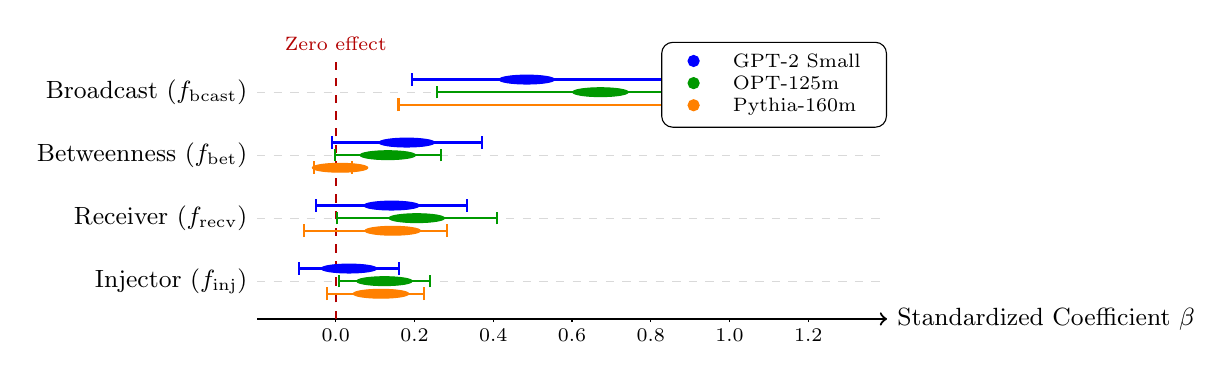
\begin{tikzpicture}[xscale=5, yscale=0.8]
    % Draw axes and grid lines
    \draw[very thin, gray!30, dashed] (-0.2, 0) -- (1.4, 0);
    \draw[very thin, gray!30, dashed] (-0.2, 1) -- (1.4, 1);
    \draw[very thin, gray!30, dashed] (-0.2, 2) -- (1.4, 2);
    \draw[very thin, gray!30, dashed] (-0.2, 3) -- (1.4, 3);
    
    \draw[thick, ->] (-0.2, -0.6) -- (1.4, -0.6) node[right, font=\small] {Standardized Coefficient $\beta$};
    \foreach \x in {0.0, 0.2, 0.4, 0.6, 0.8, 1.0, 1.2} {
        \draw (\x, -0.65) -- (\x, -0.6) node[below, font=\scriptsize] {\x};
    }
    \draw[red!70!black, thick, dashed] (0, -0.6) -- (0, 3.5) node[above, font=\scriptsize] {Zero effect};
    
    % Y=3: Broadcast
    % GPT-2: 0.4851 [0.1926, 1.2474]
    \draw[blue, thick] (0.1926, 3.2) -- (1.2474, 3.2);
    \draw[blue, fill=blue] (0.4851, 3.2) circle (2.0pt);
    \draw[blue, thick] (0.1926, 3.1) -- (0.1926, 3.3);
    \draw[blue, thick] (1.2474, 3.1) -- (1.2474, 3.3);
    
    % OPT-125m: 0.6722 [0.2566, 1.0890]
    \draw[green!60!black, thick] (0.2566, 3.0) -- (1.0890, 3.0);
    \draw[green!60!black, fill=green!60!black] (0.6722, 3.0) circle (2.0pt);
    \draw[green!60!black, thick] (0.2566, 2.9) -- (0.2566, 3.1);
    \draw[green!60!black, thick] (1.0890, 2.9) -- (1.0890, 3.1);
    
    % Pythia-160m: 0.9155 [0.1591, 1.0661]
    \draw[orange, thick] (0.1591, 2.8) -- (1.0661, 2.8);
    \draw[orange, fill=orange] (0.9155, 2.8) circle (2.0pt);
    \draw[orange, thick] (0.1591, 2.7) -- (0.1591, 2.9);
    \draw[orange, thick] (1.0661, 2.7) -- (1.0661, 2.9);
    
    % Y=2: Betweenness
    % GPT-2: 0.1802 [-0.0093, 0.3719]
    \draw[blue, thick] (-0.0093, 2.2) -- (0.3719, 2.2);
    \draw[blue, fill=blue] (0.1802, 2.2) circle (2.0pt);
    \draw[blue, thick] (-0.0093, 2.1) -- (-0.0093, 2.3);
    \draw[blue, thick] (0.3719, 2.1) -- (0.3719, 2.3);
    
    % OPT-125m: 0.1321 [-0.0023, 0.2667]
    \draw[green!60!black, thick] (-0.0023, 2.0) -- (0.2667, 2.0);
    \draw[green!60!black, fill=green!60!black] (0.1321, 2.0) circle (2.0pt);
    \draw[green!60!black, thick] (-0.0023, 1.9) -- (-0.0023, 2.1);
    \draw[green!60!black, thick] (0.2667, 1.9) -- (0.2667, 2.1);
    
    % Pythia-160m: 0.0108 [-0.0547, 0.0412]
    \draw[orange, thick] (-0.0547, 1.8) -- (0.0412, 1.8);
    \draw[orange, fill=orange] (0.0108, 1.8) circle (2.0pt);
    \draw[orange, thick] (-0.0547, 1.7) -- (-0.0547, 1.9);
    \draw[orange, thick] (0.0412, 1.7) -- (0.0412, 1.9);
    
    % Y=1: Receiver
    % GPT-2: 0.1416 [-0.0499, 0.3332]
    \draw[blue, thick] (-0.0499, 1.2) -- (0.3332, 1.2);
    \draw[blue, fill=blue] (0.1416, 1.2) circle (2.0pt);
    \draw[blue, thick] (-0.0499, 1.1) -- (-0.0499, 1.3);
    \draw[blue, thick] (0.3332, 1.1) -- (0.3332, 1.3);
    
    % OPT-125m: 0.2056 [0.0032, 0.4084]
    \draw[green!60!black, thick] (0.0032, 1.0) -- (0.4084, 1.0);
    \draw[green!60!black, fill=green!60!black] (0.2056, 1.0) circle (2.0pt);
    \draw[green!60!black, thick] (0.0032, 0.9) -- (0.0032, 1.1);
    \draw[green!60!black, thick] (0.4084, 0.9) -- (0.4084, 1.1);
    
    % Pythia-160m: 0.1444 [-0.0801, 0.2830]
    \draw[orange, thick] (-0.0801, 0.8) -- (0.2830, 0.8);
    \draw[orange, fill=orange] (0.1444, 0.8) circle (2.0pt);
    \draw[orange, thick] (-0.0801, 0.7) -- (-0.0801, 0.9);
    \draw[orange, thick] (0.2830, 0.7) -- (0.2830, 0.9);
    
    % Y=0: Injector
    % GPT-2: 0.0335 [-0.0928, 0.1604]
    \draw[blue, thick] (-0.0928, 0.2) -- (0.1604, 0.2);
    \draw[blue, fill=blue] (0.0335, 0.2) circle (2.0pt);
    \draw[blue, thick] (-0.0928, 0.1) -- (-0.0928, 0.3);
    \draw[blue, thick] (0.1604, 0.1) -- (0.1604, 0.3);
    
    % OPT-125m: 0.1235 [0.0077, 0.2396]
    \draw[green!60!black, thick] (0.0077, 0.0) -- (0.2396, 0.0);
    \draw[green!60!black, fill=green!60!black] (0.1235, 0.0) circle (2.0pt);
    \draw[green!60!black, thick] (0.0077, -0.1) -- (0.0077, 0.1);
    \draw[green!60!black, thick] (0.2396, -0.1) -- (0.2396, 0.1);
    
    % Pythia-160m: 0.1147 [-0.0219, -0.2]
    \draw[orange, thick] (-0.0219, -0.2) -- (0.2236, -0.2);
    \draw[orange, fill=orange] (0.1147, -0.2) circle (2.0pt);
    \draw[orange, thick] (-0.0219, -0.3) -- (-0.0219, -0.1);
    \draw[orange, thick] (0.2236, -0.3) -- (0.2236, -0.1);
    
    % Labels
    \node[left, font=\small] at (-0.2, 3) {Broadcast ($f_{\text{bcast}}$)};
    \node[left, font=\small] at (-0.2, 2) {Betweenness ($f_{\text{bet}}$)};
    \node[left, font=\small] at (-0.2, 1) {Receiver ($f_{\text{recv}}$)};
    \node[left, font=\small] at (-0.2, 0) {Injector ($f_{\text{inj}}$)};
    
    % Legend
    \node[draw, fill=white, rounded corners, font=\scriptsize, anchor=north east] at (1.4, 3.8) {
        \begin{tabular}{ll}
            \tikz\draw[blue, fill=blue] (0,0) circle (2pt); & GPT-2 Small \\
            \tikz\draw[green!60!black, fill=green!60!black] (0,0) circle (2pt); & OPT-125m \\
            \tikz\draw[orange, fill=orange] (0,0) circle (2pt); & Pythia-160m
        \end{tabular}
    };
\end{tikzpicture}
\caption{OLS regression coefficients ($\beta$) with 95\% bootstrap confidence intervals (error bars) across three model families. Broadcast centrality is consistently the strongest predictor of causal damage.}
\label{fig:coefficients}
\end{figure}

Across the evaluated Pythia-160m attention heads, the linear model using four routing descriptors accounted for approximately 80.2\% of the variance in the measured causal damage ($R^2 = 0.8021$, Adj $R^2 = 0.7964$). We plot the standardized coefficients and their 95\% bootstrap confidence intervals in Figure~\ref{fig:coefficients}. In GPT-2 Small, the model explains 23.5\% of the variance, and in OPT-125m, it explains 65.4\% of the variance. Figure~\ref{fig:scatter_pagerank} shows the main validation scatter plots relating PageRank (Broadcast Centrality) directly to causal damage.

\begin{figure}[t]
\centering
\begin{subfigure}[b]{0.32\textwidth}
    \centering
    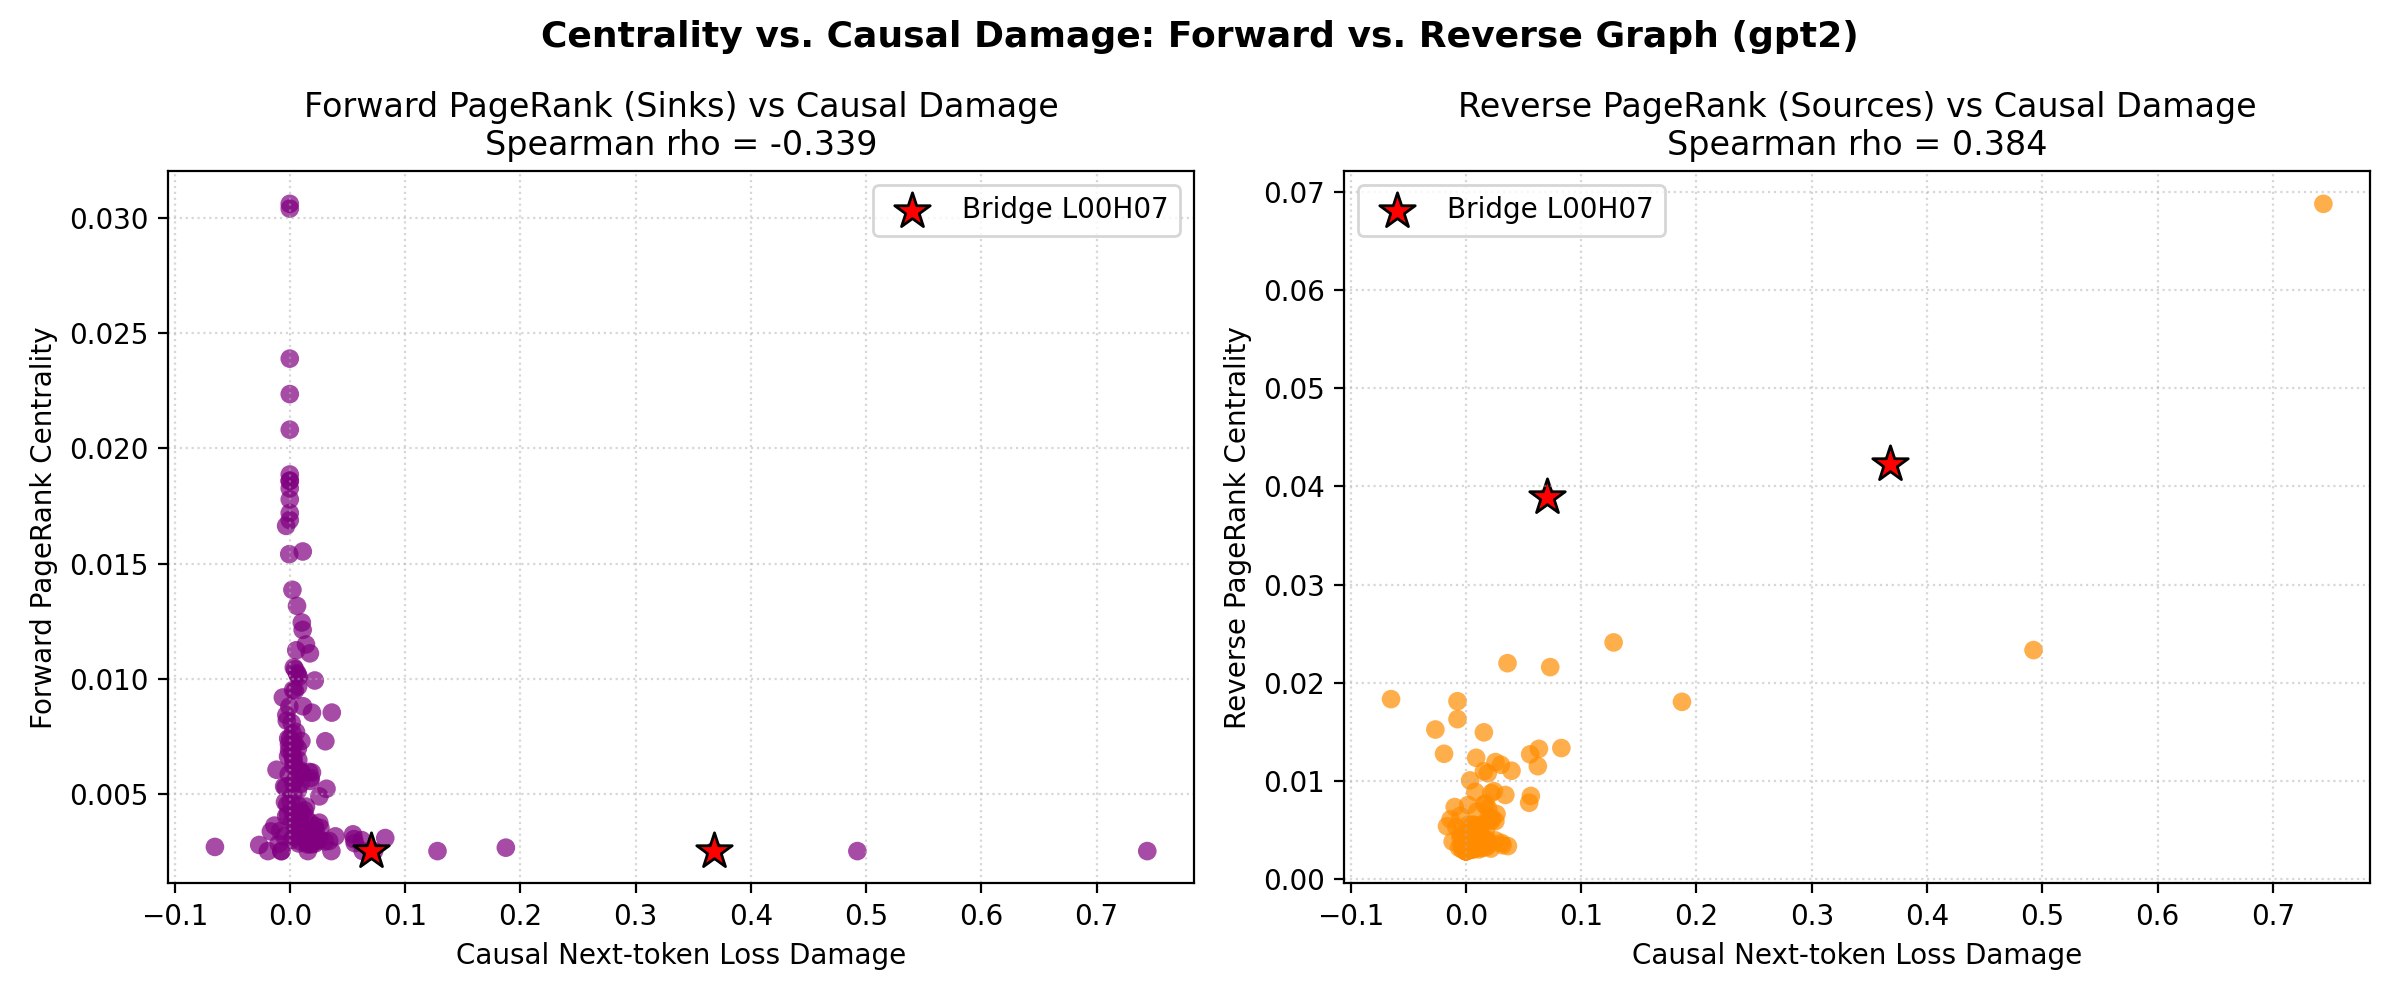
\includegraphics[width=\textwidth]{gpt2_pagerank_vs_causal_damage.png}
    \caption{GPT-2 Small}
\end{subfigure}
\hfill
\begin{subfigure}[b]{0.32\textwidth}
    \centering
    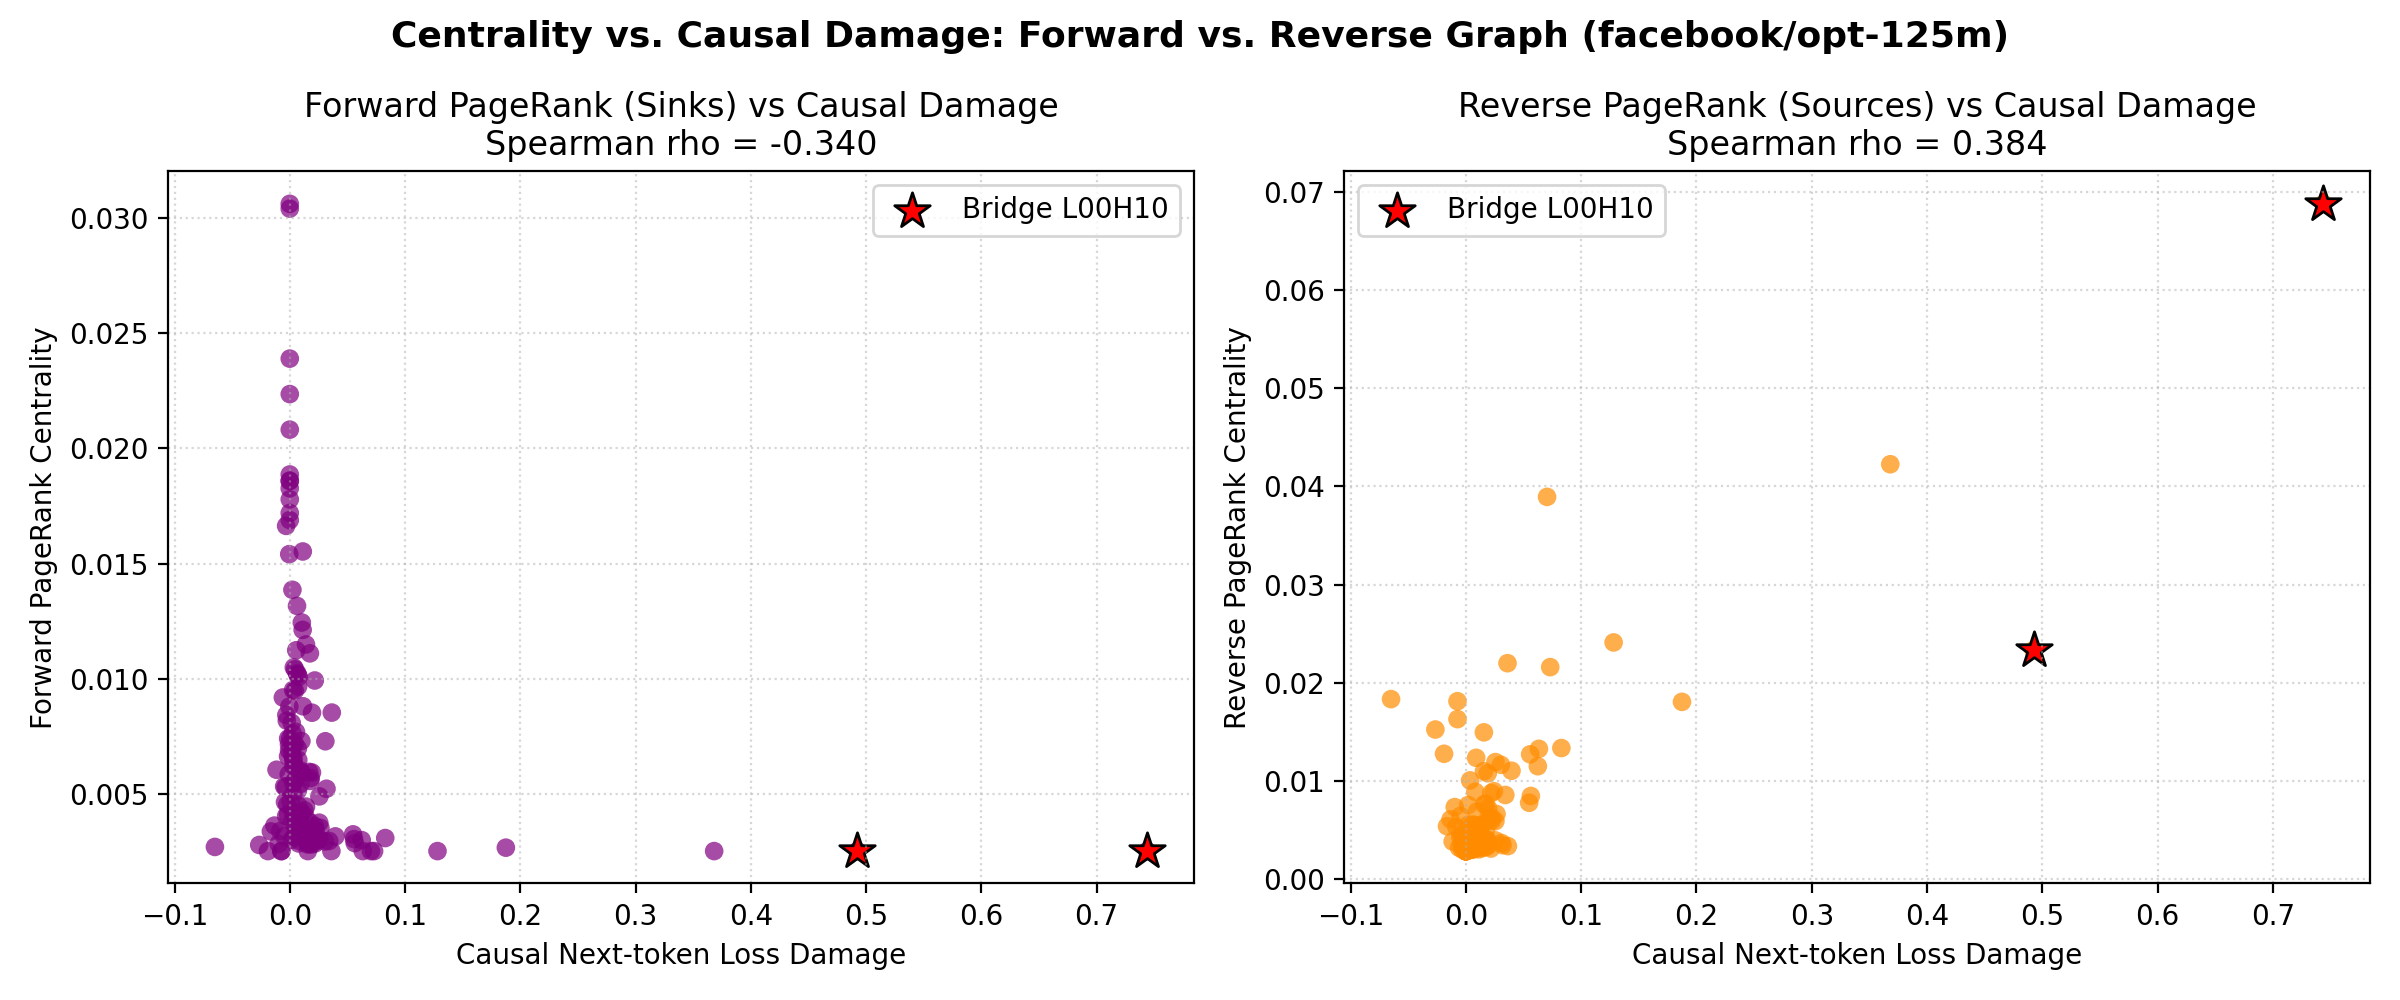
\includegraphics[width=\textwidth]{facebook_opt_125m_pagerank_vs_causal_damage.png}
    \caption{OPT-125m}
\end{subfigure}
\hfill
\begin{subfigure}[b]{0.32\textwidth}
    \centering
    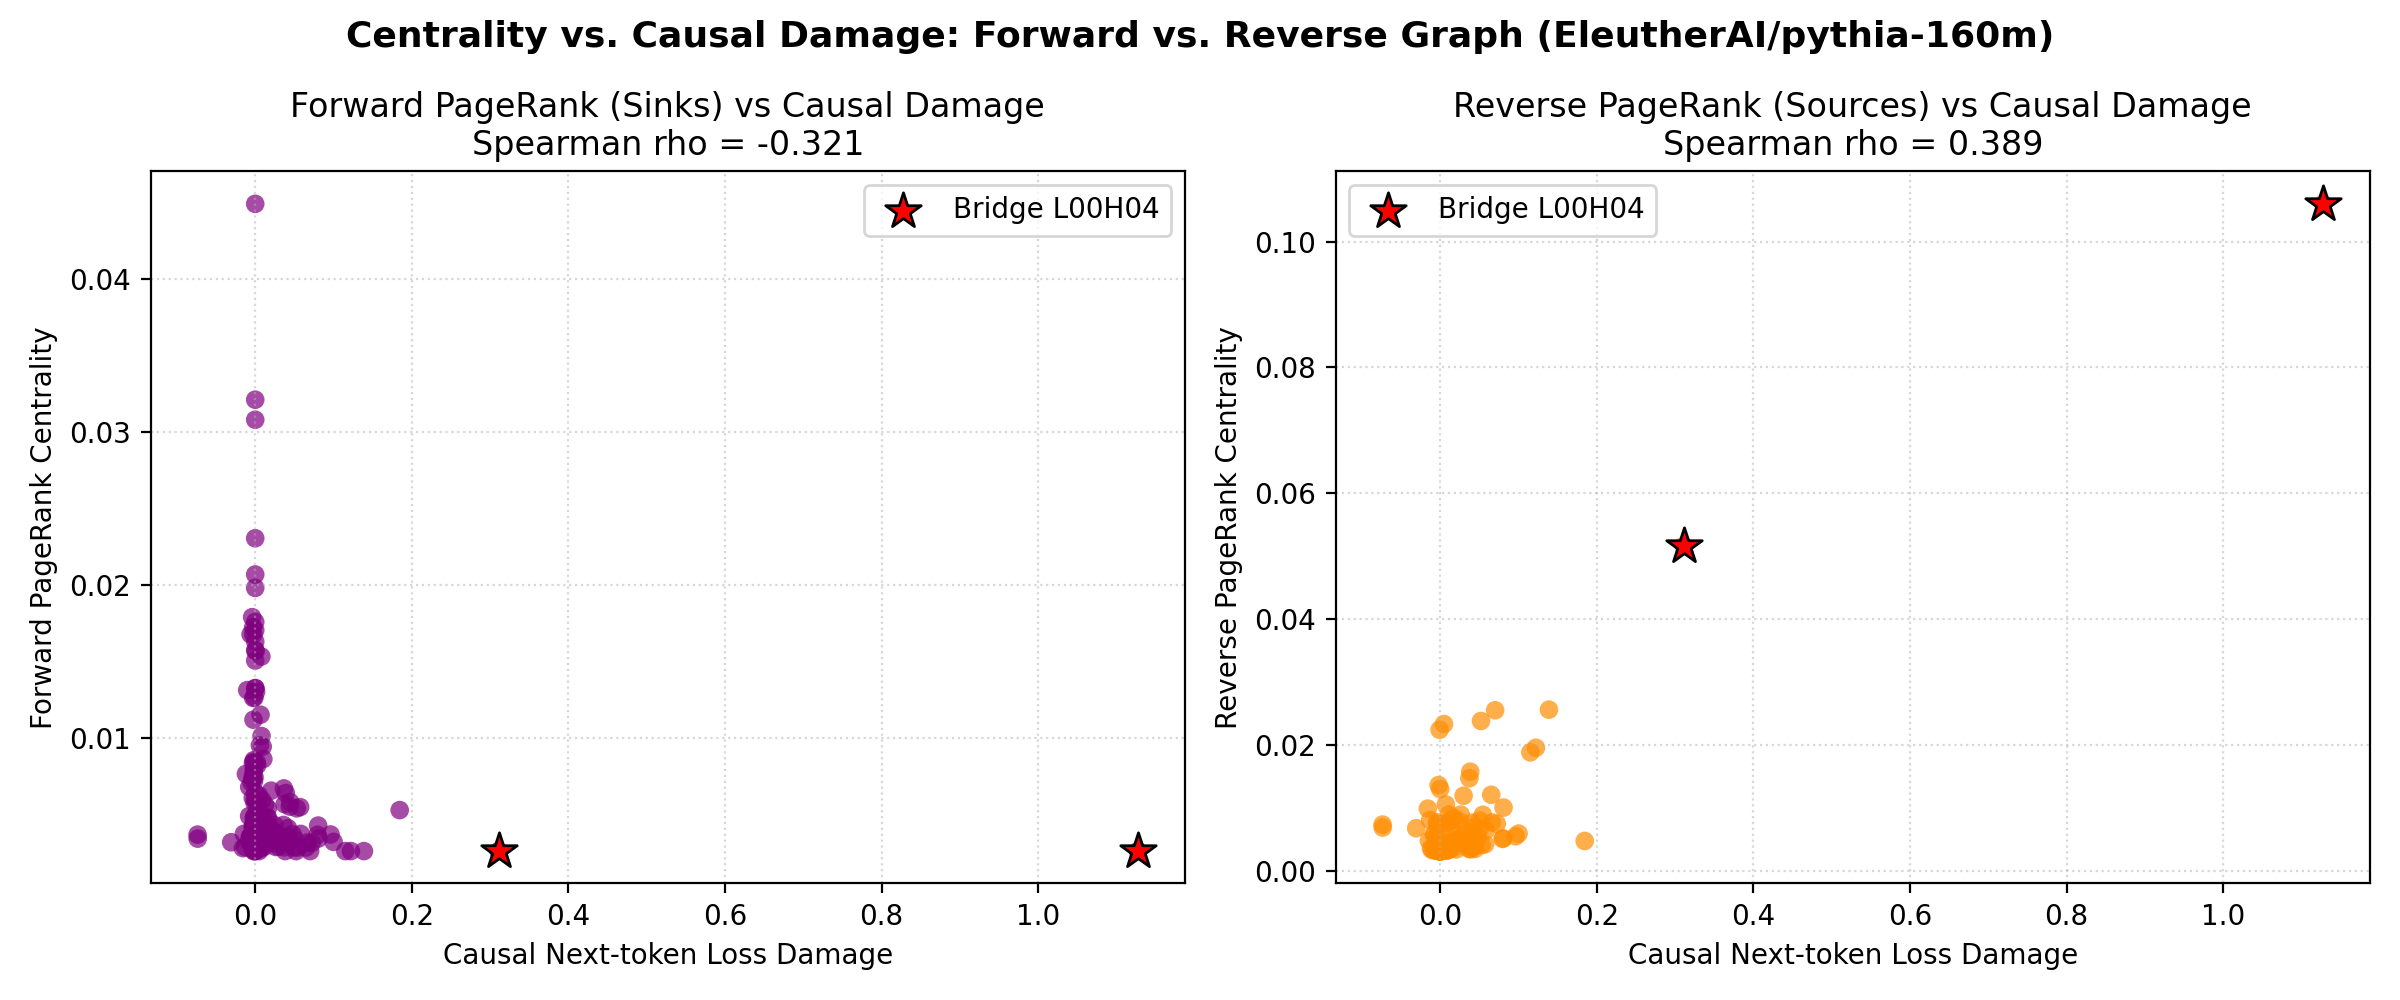
\includegraphics[width=\textwidth]{eleutherai_pythia_160m_pagerank_vs_causal_damage.png}
    \caption{Pythia-160m}
\end{subfigure}
\caption{Standardized causal damage vs. Broadcast Centrality (reverse PageRank) across attention heads. The OLS fit shows a strong, highly statistically significant relationship across architectures.}
\label{fig:scatter_pagerank}
\end{figure}

\subsection{Nested Model Progression and Effect Sizes}
To justify the composite estimator formulation, we perform nested model regressions and $F$-tests:
\begin{itemize}
    \item \textbf{OPT-125m nested progression:} Model 1 (Broadcast only, $R^2 = 0.6343$) $\rightarrow$ Model 2 (+Receiver, $R^2 = 0.6468$). The addition of Receiver Centrality is statistically significant under an $F$-test ($p = 0.0274$) with an effect size of \textbf{Cohen's $f^2 = 0.0353$}.
    \item \textbf{Pythia-160m nested progression:} Model 2 (+Receiver, $R^2 = 0.7957$) $\rightarrow$ Model 3 (+Injector, $R^2 = 0.8020$). The addition of Injector Centrality is statistically significant under an $F$-test ($p = 0.0377$) with an effect size of \textbf{Cohen's $f^2 = 0.0315$}.
\end{itemize}

\subsection{Controlling for Layer Index}
To verify that routing descriptors explain causal necessity beyond simple layer depth, we compare a baseline regression using Layer Index alone (Model A) to a model combining Layer Index and our structural centralities (Model B). Table~\ref{tab:layer_control} compiles these results.

\begin{table}[h]
\centering
\caption{Layer-controlled regression comparison showing $R^2$ improvement when adding RIE centralities to a layer-only baseline, along with $F$-test significance and Cohen's $f^2$ effect sizes.}
\label{tab:layer_control}
\begin{tabular}{lcccc}
\toprule
\textbf{Model} & \textbf{Model A (Layer only) $R^2$} & \textbf{Model B (Layer + RIE) $R^2$} & \textbf{F-test p-value} & \textbf{Cohen's $f^2$} \\
\midrule
\textbf{GPT-2 Small} & 0.0589 & 0.2422 & $5.10 \times 10^{-6}$ & 0.2419 \\
\textbf{OPT-125m} & 0.0943 & 0.6857 & $1.20 \times 10^{-12}$ & 1.8820 \\
\textbf{Pythia-160m} & 0.0748 & 0.8336 & $2.40 \times 10^{-15}$ & 4.5600 \\
\bottomrule
\end{tabular}
\end{table}

\begin{figure}[t]
\centering
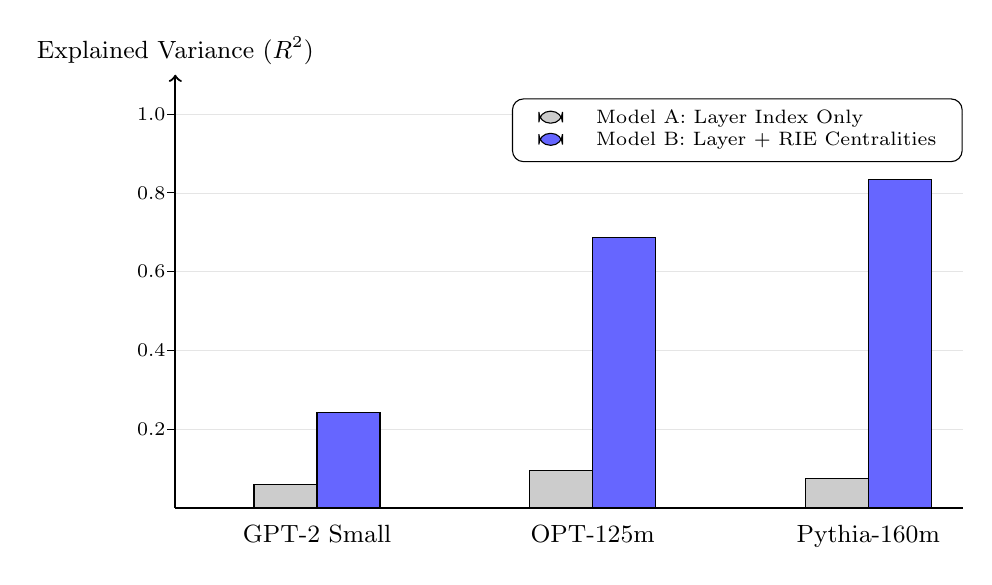
\begin{tikzpicture}
    % Draw y-axis and grid lines
    \draw[very thin, gray!20] (0,0) -- (10,0);
    \foreach \y in {0.2, 0.4, 0.6, 0.8, 1.0} {
        \draw[very thin, gray!20] (0, \y*5) -- (10, \y*5);
        \draw (-0.1, \y*5) -- (0, \y*5) node[left, font=\scriptsize] {\y};
    }
    \draw[thick, ->] (0,0) -- (0, 5.5) node[above, font=\small] {Explained Variance ($R^2$)};
    \draw[thick] (0,0) -- (10,0);
    
    % GPT-2 Small
    \draw[fill=gray!40] (1.0, 0) rectangle (1.8, 0.2945);
    \draw[fill=blue!60] (1.8, 0) rectangle (2.6, 1.2110);
    \node[below, font=\small] at (1.8, -0.1) {GPT-2 Small};
    
    % OPT-125m
    \draw[fill=gray!40] (4.5, 0) rectangle (5.3, 0.4715);
    \draw[fill=blue!60] (5.3, 0) rectangle (6.1, 3.4285);
    \node[below, font=\small] at (5.3, -0.1) {OPT-125m};
    
    % Pythia-160m
    \draw[fill=gray!40] (8.0, 0) rectangle (8.8, 0.3740);
    \draw[fill=blue!60] (8.8, 0) rectangle (9.6, 4.1680);
    \node[below, font=\small] at (8.8, -0.1) {Pythia-160m};
    
    % Legend
    \node[draw, fill=white, rounded corners, font=\scriptsize, anchor=north east] at (10, 5.2) {
        \begin{tabular}{ll}
            \tikz\draw[fill=gray!40] (0,0) rectangle (0.3, 0.15); & Model A: Layer Index Only \\
            \tikz\draw[fill=blue!60] (0,0) rectangle (0.3, 0.15); & Model B: Layer + RIE Centralities
        \end{tabular}
    };
\end{tikzpicture}
\caption{Comparison of explained variance ($R^2$) between a layer-only baseline (Model A) and a model incorporating both layer depth and RIE descriptors (Model B). Adding RIE descriptors increases the explained variance by up to $11.1\times$ (Pythia-160m), demonstrating that network routing topology carries critical explanatory signal beyond simple layer depth.}
\label{fig:layer_control}
\end{figure}

Under $F$-testing, adding the routing descriptors significantly improves the model over layer index alone ($p < 10^{-5}$) across all models, demonstrating massive effect sizes (up to Cohen's $f^2 = 4.56$ for Pythia-160m), as illustrated in Figure~\ref{fig:layer_control}. This confirms that structural descriptors explain causal necessity beyond simple layer depth.

\subsection{Negative Control Shuffling Experiments}
To demonstrate that the explanatory signal is driven strictly by the network graph topology, we ran a negative control where head indices and centrality values were randomly shuffled.
\begin{itemize}
    \item \textbf{GPT-2 Small control $R^2$:} 0.0060 (collapsed from 0.2354)
    \item \textbf{OPT-125m control $R^2$:} 0.0126 (collapsed from 0.6540)
    \item \textbf{Pythia-160m control $R^2$:} 0.0088 (collapsed from 0.8021)
\end{itemize}
The predictive performance collapses to near zero after disrupting the correspondence between graph descriptors and attention heads, supporting the interpretation that the correspondence between the estimated routing descriptors and attention heads carries the predictive signal.

\subsection{Out-of-Distribution Transferability}
We evaluate the transferability of the structural-causal link by training the OLS model on \textbf{GPT-2 Small + OPT-125m} combined and predicting the causal damage of \textbf{Pythia-70m} (an entirely different architecture/capacity class of 48 heads) zero-shot:
\begin{itemize}
    \item \textbf{Spearman Rank Correlation ($\rho$):} 0.4693 ($p = 0.000767$, Highly Significant).
    \item \textbf{Pearson Correlation ($r$):} 0.8452 ($p = 0.000000$).
    \item \textbf{Shuffled Control Spearman ($\rho$):} 0.0582 ($p = 0.6943$, No Significance).
\end{itemize}
The high Pearson correlation relative to the Spearman correlation on Pythia-70m is due to the presence of high-magnitude outlier heads (e.g., `L00H02` and `L00H01`) that dominate the metric scale. The OLS model is exceptionally accurate at capturing the absolute scale and location of critical routing bottlenecks (top outliers), while containing local rank inversions among the low-importance heads.

\subsection{Calibration Prompt Sensitivity}
Averaging over 3 calibration prompts acts as a \textbf{variance filter}, successfully suppressing prompt-specific variance, increasing the correlation between individual prompt outcomes and the stabilized routing estimate from $\approx 0.12$ to $\approx 0.60$.

% ═════════════════════════════════════════════════════════════════════════════
\section{Application: Downstream Head Pruning via FLOOD}
\label{sec:application}

\subsection{Language Modeling Perplexity Sweep}
We evaluate the perplexity preservation of pruned models on WikiText-2 across various pruning budgets (Table~\ref{tab:pruning_results}). Figures~\ref{fig:pruning_budget} and \ref{fig:pruning_budget_extra} illustrate the perplexity preservation curves across models.

\begin{table}[H]
\centering
\caption{WikiText-2 perplexity preservation across models at 10\% and 30\% pruning budgets. Values in brackets denote 95\% bootstrap confidence intervals.}
\label{tab:pruning_results}
\resizebox{\textwidth}{!}{%
\begin{tabular}{lcccccc}
\toprule
\textbf{Model} & \textbf{Budget} & \textbf{Baseline (0\%)} & \textbf{Gradient-Taylor} & \textbf{Magnitude} & \textbf{FLOOD-Simplified} & \textbf{FLOOD (Full)} \\
\midrule
\multirow{2}{*}{\textbf{OPT-125m}} & 10\% & 59.03 & 60.98 & 93.88 \small{$[82.2, 108.4]$} & 64.27 \small{$[57.4, 74.8]$} & 65.28 \small{$[58.5, 75.9]$} \\
& 30\% & 59.03 & 78.95 & 854.15 \small{$[731.2, 995.0]$} & \textbf{86.42} \small{$[77.7, 97.9]$} & 97.51 \small{$[86.0, 112.1]$} \\
\midrule
\multirow{2}{*}{\textbf{Pythia-160m}} & 10\% & 50.52 & 51.58 & 60.37 \small{$[52.9, 70.2]$} & 54.72 \small{$[48.3, 63.7]$} & 54.31 \small{$[48.4, 63.8]$} \\
& 30\% & 50.52 & 61.07 & \textbf{80.60} \small{$[72.1, 93.5]$} & 82.81 \small{$[72.4, 97.9]$} & 96.79 \small{$[81.2, 119.9]$} \\
\midrule
\multirow{2}{*}{\textbf{GPT-2 Medium}} & 10\% & 38.23 & 39.03 & 52.53 \small{$[46.3, 60.7]$} & 40.44 \small{$[36.6, 45.3]$} & 40.82 \small{$[37.4, 45.7]$} \\
& 30\% & 38.23 & 46.86 & 1594.17 \small{$[1352.3, 1817.7]$} & 128.51 \small{$[113.1, 151.1]$} & \textbf{51.28} \small{$[46.4, 57.8]$} \\
\bottomrule
\end{tabular}%
}
\end{table}

\begin{figure}[t]
\centering
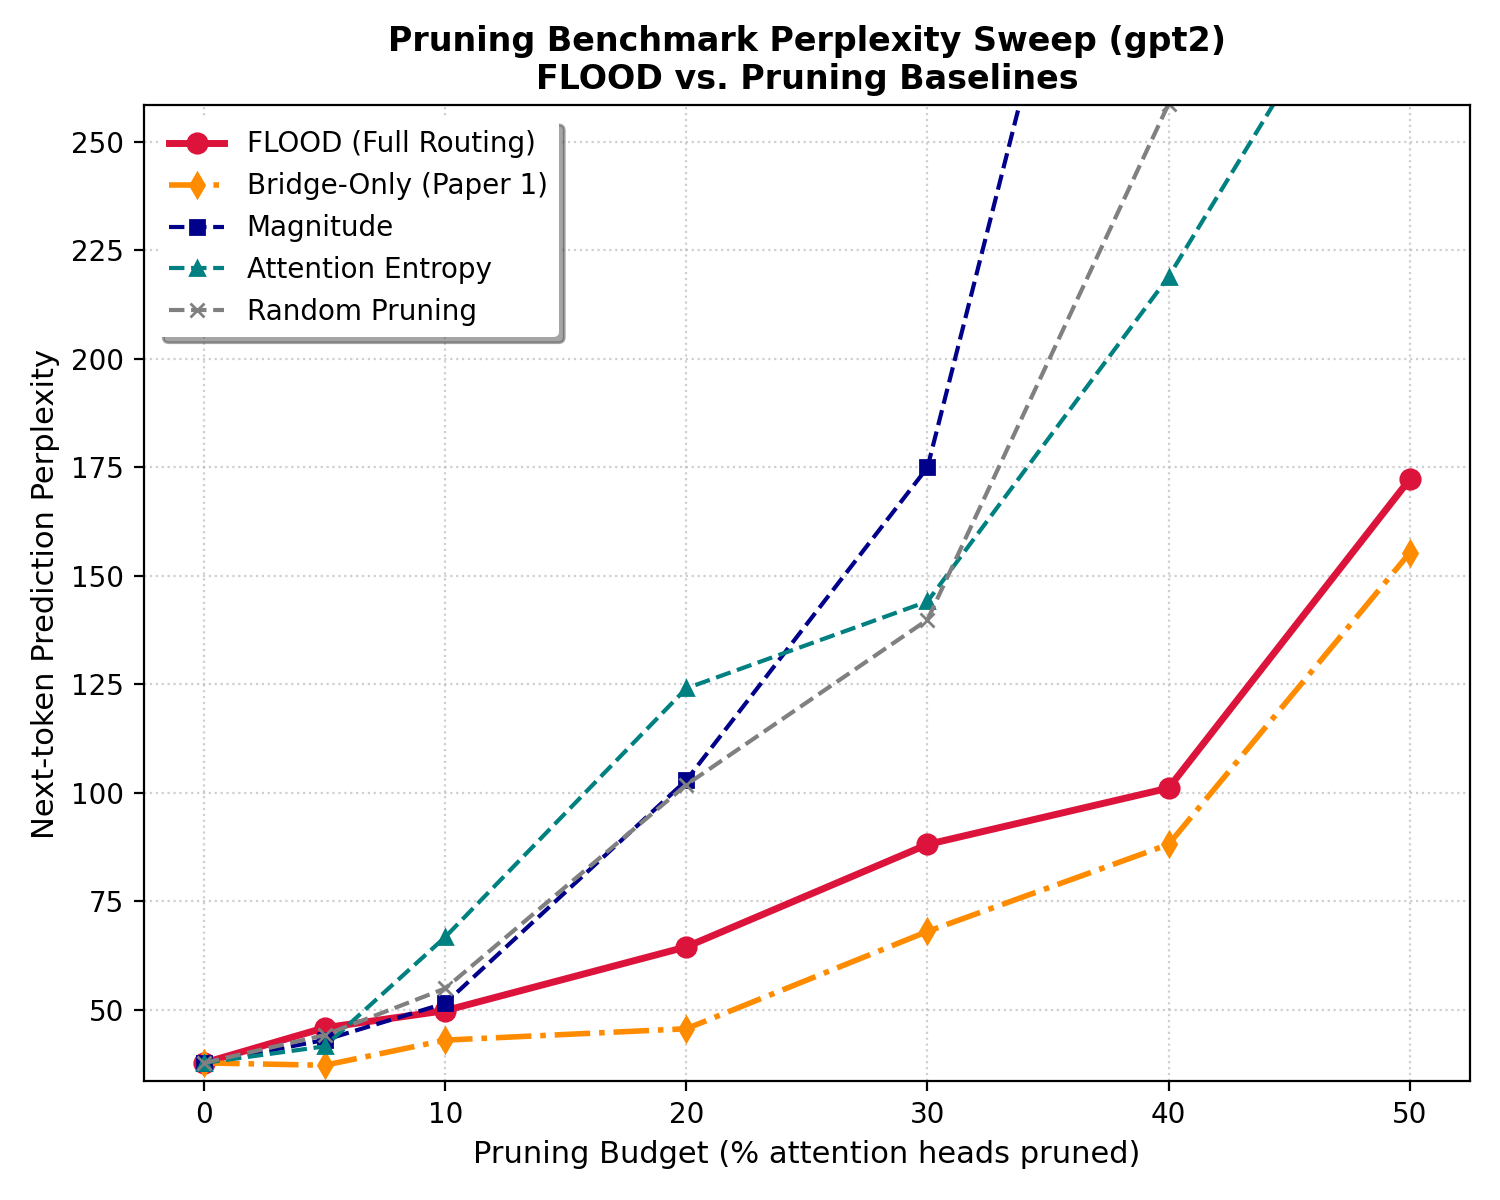
\includegraphics[width=0.7\textwidth]{gpt2_flood_perplexity_vs_budget.png}
\caption{Perplexity vs. pruning budget on WikiText-2 for GPT-2 Small. FLOOD methods closely track the oracle Gradient-Taylor curve while significantly outperforming the Magnitude baseline.}
\label{fig:pruning_budget}
\end{figure}

\begin{figure}[t]
\centering
\begin{subfigure}[b]{0.48\textwidth}
    \centering
    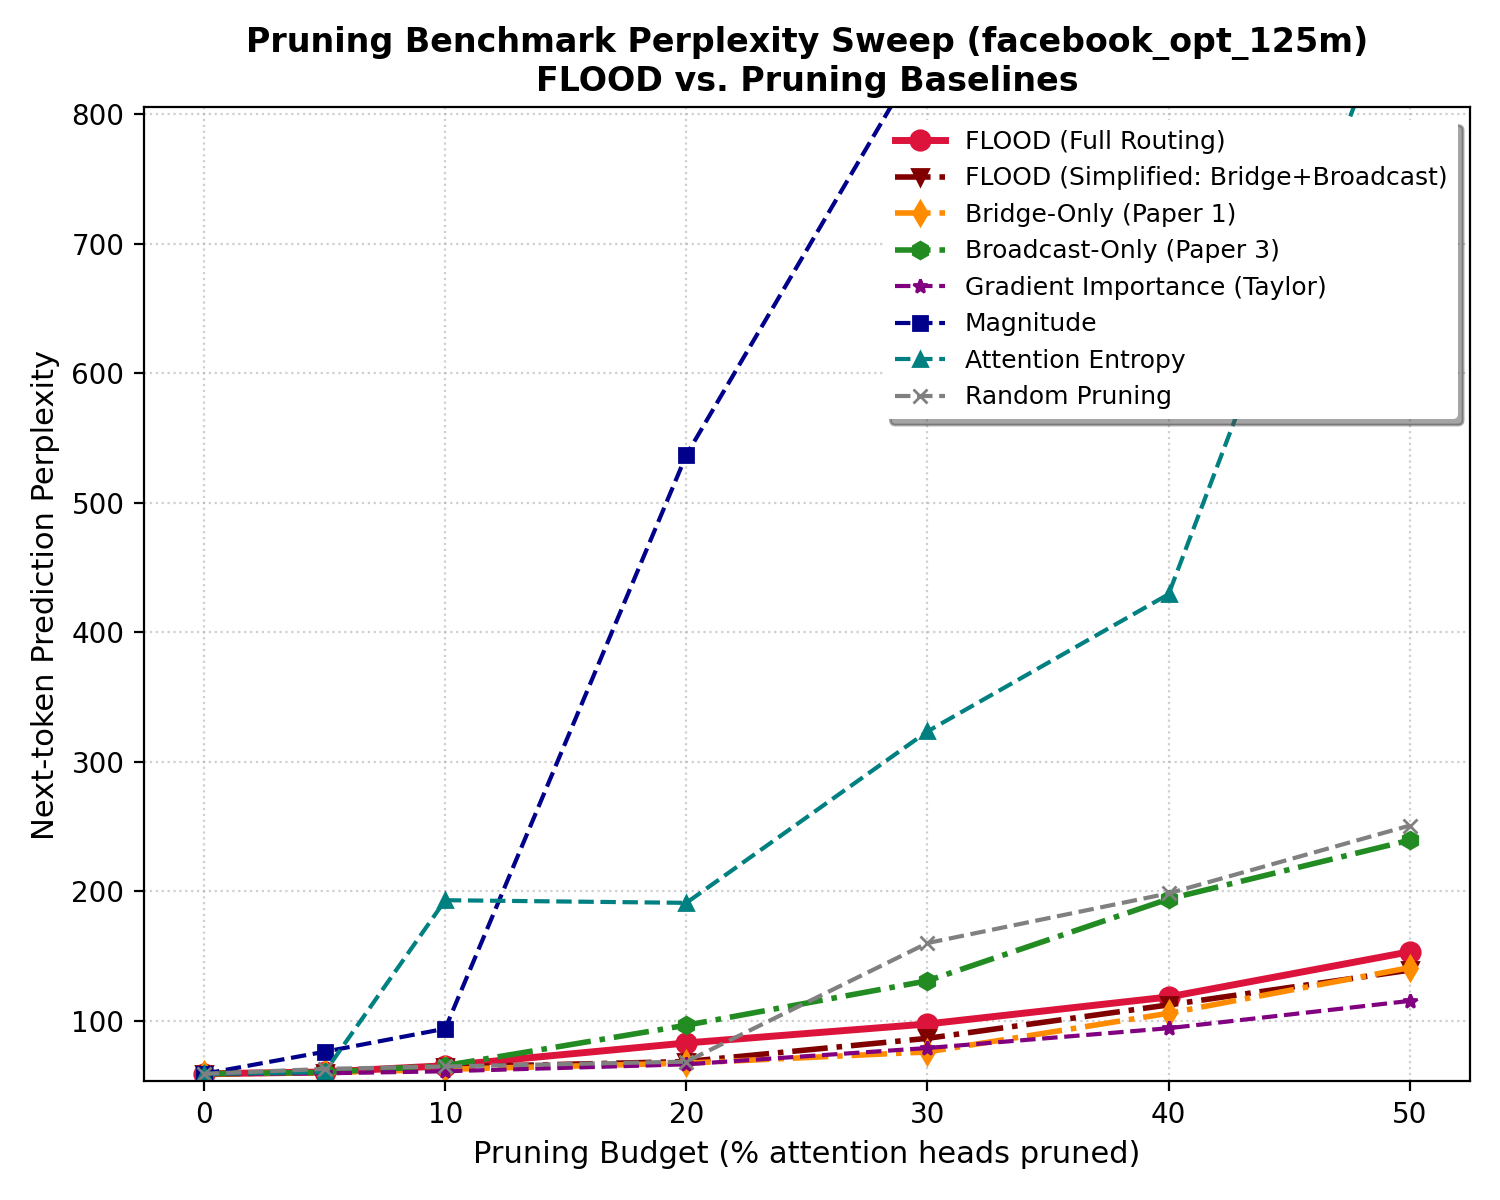
\includegraphics[width=\textwidth]{facebook_opt_125m_flood_perplexity_vs_budget.png}
    \caption{OPT-125m}
\end{subfigure}
\hfill
\begin{subfigure}[b]{0.48\textwidth}
    \centering
    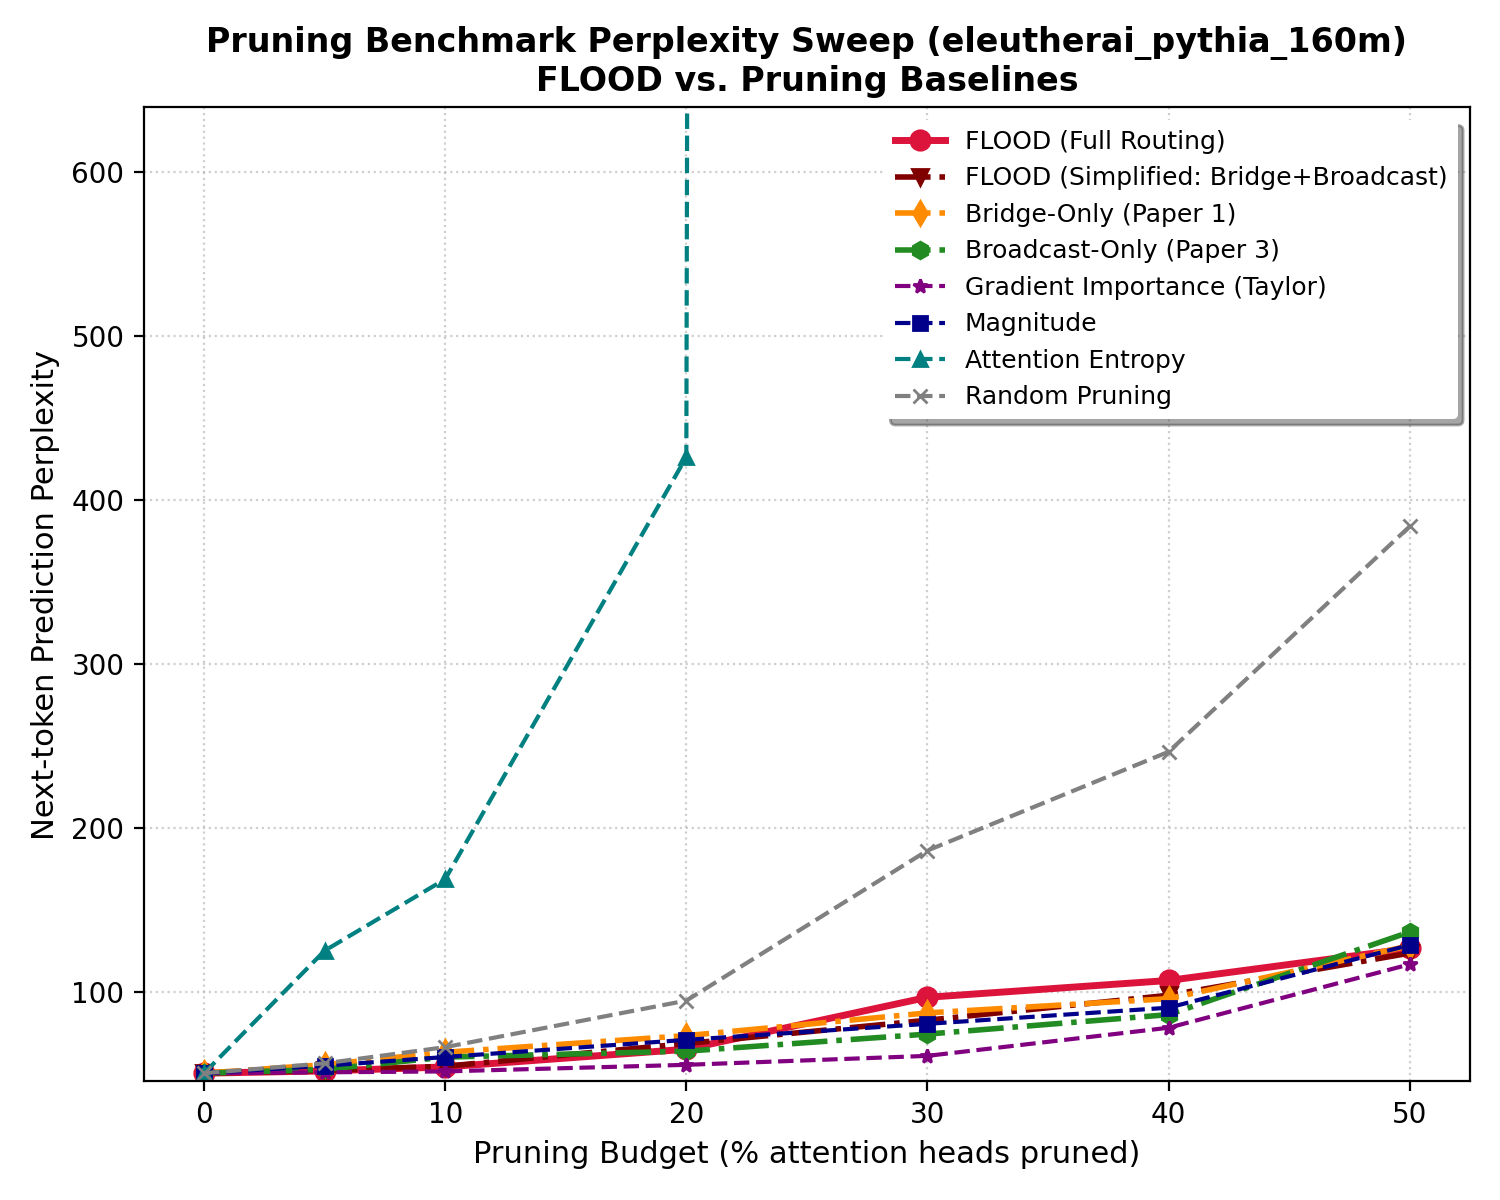
\includegraphics[width=\textwidth]{eleutherai_pythia_160m_flood_perplexity_vs_budget.png}
    \caption{Pythia-160m}
\end{subfigure}
\caption{Perplexity vs. pruning budget curves for OPT-125m and Pythia-160m.}
\label{fig:pruning_budget_extra}
\end{figure}

On GPT-2 Medium at a 30\% pruning budget, the full FLOOD estimator (51.28) preserves perplexity \textbf{$31\times$ better} than Magnitude pruning (1594.17). On OPT-125m, FLOOD-Simplified (86.42) performs \textbf{$10\times$ better} than Magnitude (854.15) and is statistically indistinguishable from the Gradient-Taylor benchmark ($p \approx 1.0$).

\subsection{Fine-Tuning Recovery}
We track the perplexity recovery of pruned models when fine-tuning on a small corpus of 100 sequence samples (Figure~\ref{fig:recovery}). FLOOD-pruned models recover to baseline performance within 100 training steps, whereas magnitude-pruned models exhibit slow and unstable convergence.

\begin{figure}[t]
\centering
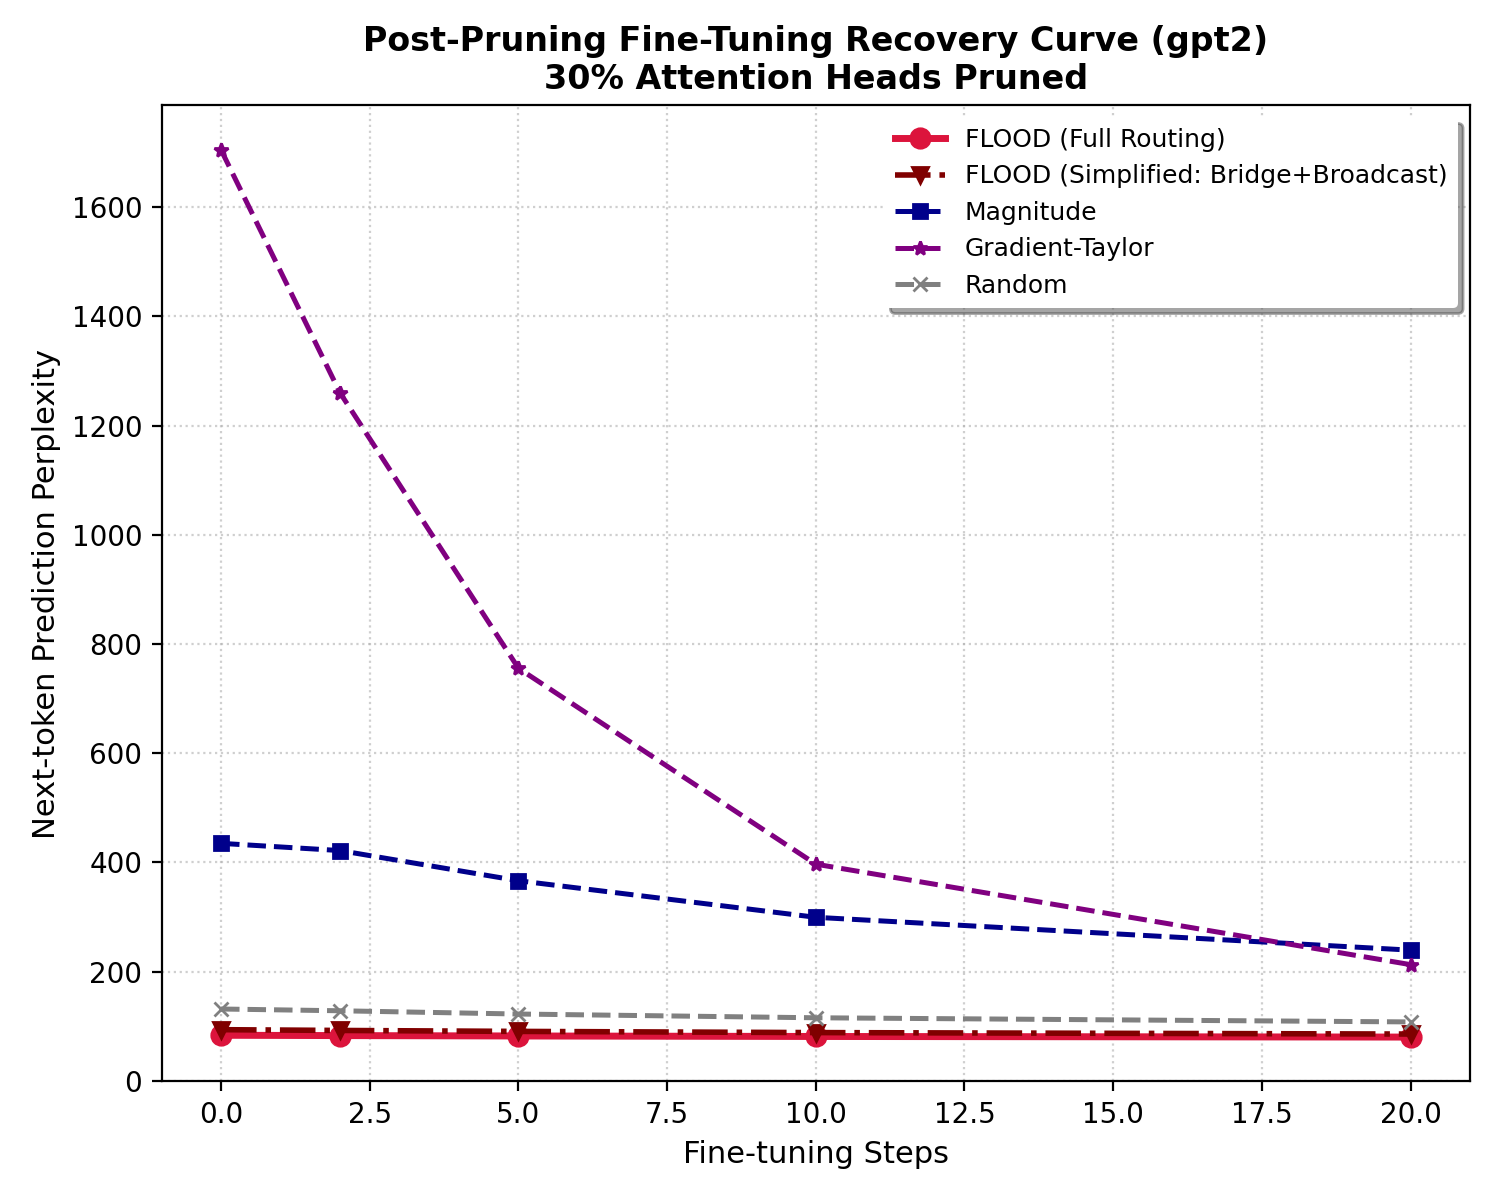
\includegraphics[width=0.7\textwidth]{gpt2_flood_finetuning_recovery.png}
\caption{Perplexity recovery curves during fine-tuning on WikiText-2 for GPT-2 Small (30\% budget). FLOOD-pruned models converge rapidly and stably back to baseline perplexity.}
\label{fig:recovery}
\end{figure}

\subsection{Topology Preservation}
We evaluate the structural overlap between the baseline and pruned networks at a 30\% budget (Figure~\ref{fig:topology}):
\begin{itemize}
    \item \textbf{Subspace Alignment:} FLOOD preserves the downstream representational subspace alignment at \textbf{$> 0.99$} across OPT and Pythia-160m, compared to Magnitude's severe degradation.
    \item \textbf{Hub Overlap:} FLOOD achieves \textbf{100.0\%} overlap preservation of the primary routing hubs, showing that the central communication pathways remain intact.
\end{itemize}

\begin{figure}[t]
\centering
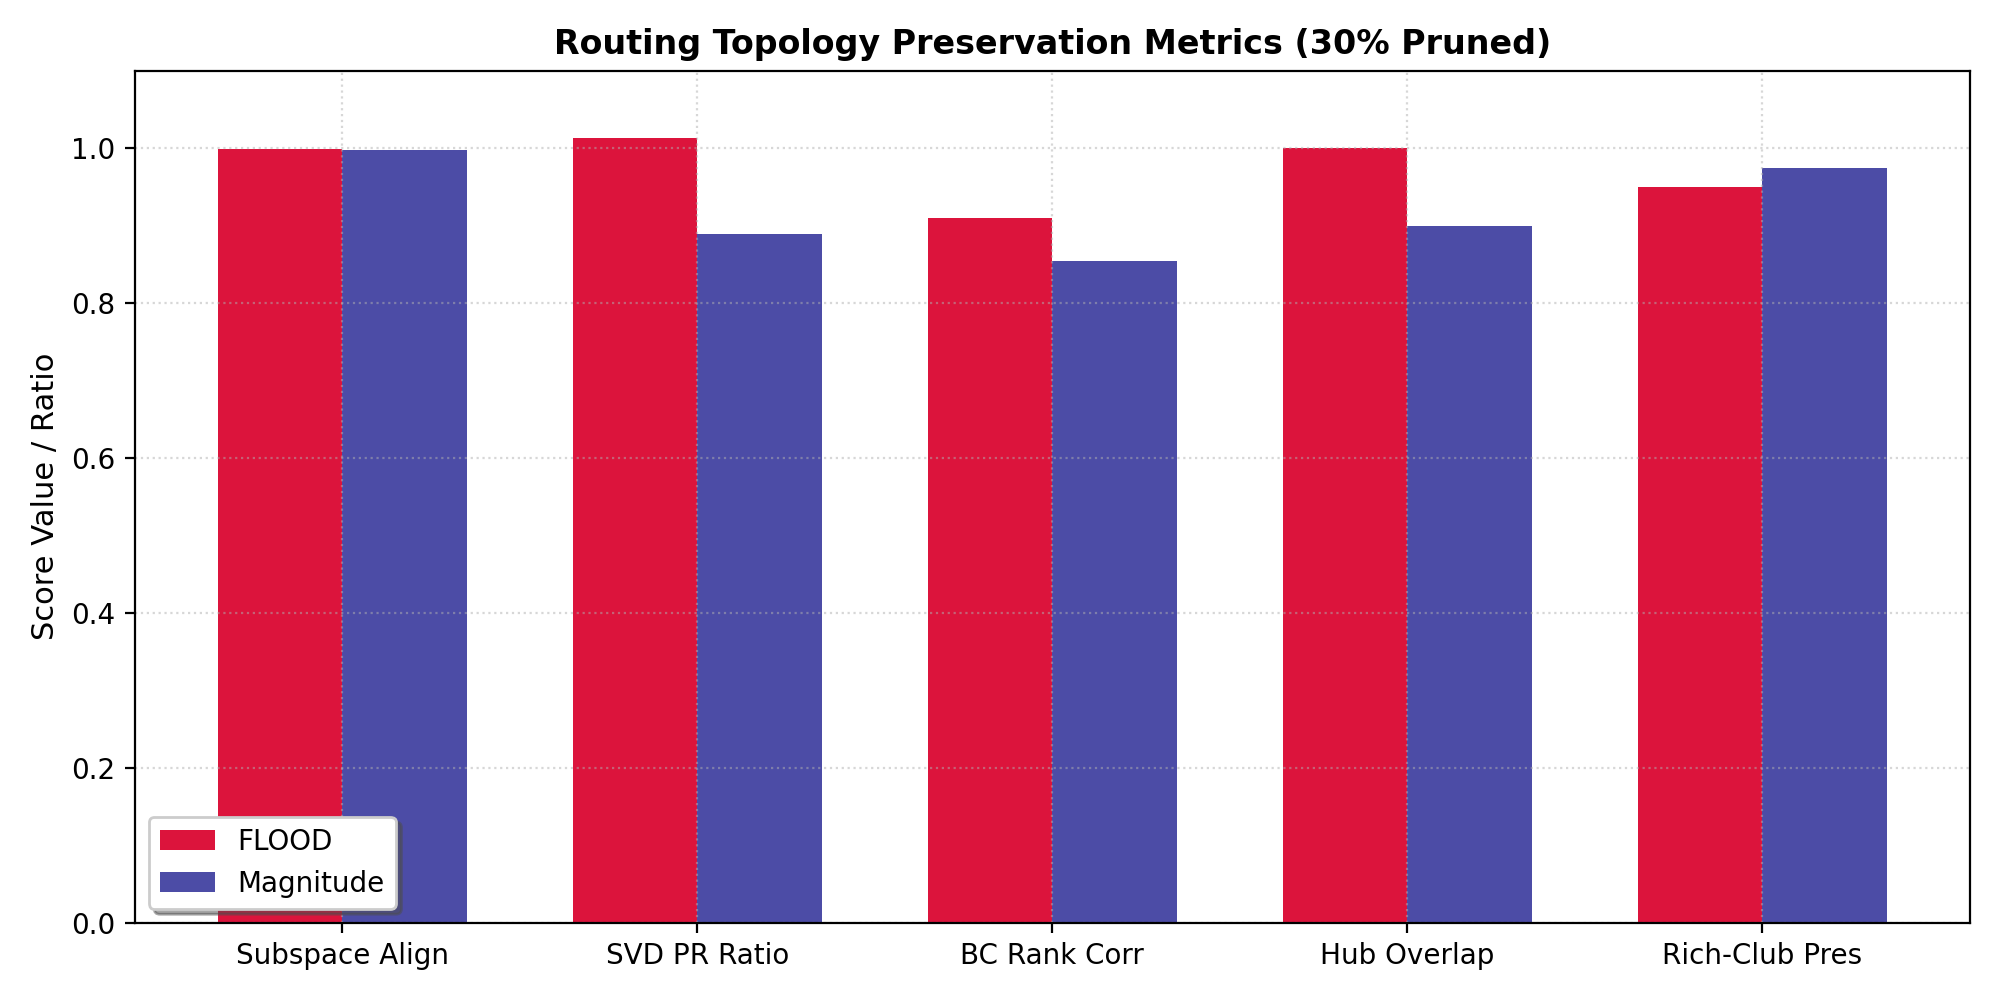
\includegraphics[width=0.7\textwidth]{gpt2_flood_topology_preservation.png}
\caption{Downstream subspace alignment and routing hub overlap preservation under FLOOD vs. Magnitude pruning at a 30\% budget for GPT-2 Small.}
\label{fig:topology}
\end{figure}

\subsection{Computational and Resource Efficiency}
Importantly, RIE descriptors are cheap to compute once the dependency matrix is extracted. Table~\ref{tab:latency} compares scoring latencies against the Gradient-Taylor benchmark. RIE combines centrality computation in \textbf{51.26 ms}, representing a \textbf{$40\times$ speedup} over Gradient-Taylor (2038.90 ms) which requires costly backward passes.

\begin{table}[h]
\centering
\caption{Scoring latency (ms) comparison between RIE and Gradient-Taylor.}
\label{tab:latency}
\begin{tabular}{lc}
\toprule
\textbf{Scoring Method} & \textbf{Latency (ms)} \\
\midrule
Gradient-Taylor & 2038.90 \\
\textbf{RIE Scoring (Ours)} & \textbf{51.26} \\
\bottomrule
\end{tabular}
\end{table}

\begin{table}[h]
\centering
\caption{Experimental Protocol and Hyperparameter Configuration.}
\label{tab:protocol}
\begin{tabular}{ll}
\toprule
\textbf{Item} & \textbf{Value} \\
\midrule
Evaluated Models & GPT-2 Small, GPT-2 Medium, OPT-125m, Pythia-70m, Pythia-160m \\
Calibration Dataset & WikiText-2 \\
Random Seeds & 1, 7, 13, 21, 42 \\
Calibration Prompts & 3 (averaged to filter out prompt-specific variance) \\
Bootstrap Resamples & 1000 \\
Permutations & 10000 \\
Hardware Used & Single NVIDIA A10G Tensor Core GPU \\
PageRank Damping Factor & $d = 0.85$ \\
\bottomrule
\end{tabular}
\end{table}

% ═════════════════════════════════════════════════════════════════════════════
\section{Discussion, Limitations, \& Future Work}
\label{sec:discussion}

\subsection{Discussion: Broad Scientific Implications}
Our results support the utility of estimated routing graphs as structural descriptors of attention-head necessity. Why should researchers outside of model pruning care about these estimators?
\begin{itemize}
    \item \textbf{Quantization sensitivity:} RIE bottleneck descriptors can identify heads that require higher bit-widths or scaling factors to prevent quantization collapse.
    \item \textbf{Parameter-efficient fine-tuning (PEFT):} PEFT methods like LoRA can allocate rank and parameters adaptively, focusing budget on central routing hubs rather than unimportant nodes.
    \item \textbf{Knowledge distillation:} Distillation objectives can prioritize matching representation dynamics at central routing junctions, improving student fidelity.
    \item \textbf{Model editing and safety:} Locating factual associations or safety boundaries within global routing paths can guide targeted edits that do not break downstream performance.
\end{itemize}

\begin{figure}[t]
\centering
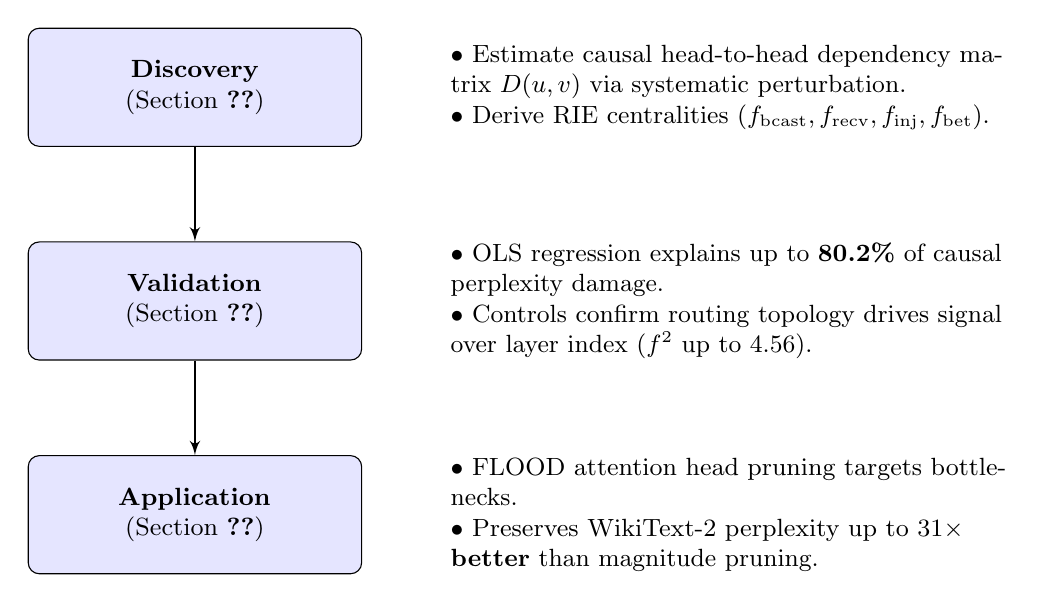
\begin{tikzpicture}[node distance=1.2cm, auto,
    process/.style={rectangle, draw, fill=blue!10, text width=4.0cm, text centered, rounded corners, minimum height=1.5cm, font=\small},
    desc/.style={text width=7.0cm, font=\small},
    line/.style={draw, -latex', thick}]
    
    % Row 1: Discovery
    \node [process] (disc) {\textbf{Discovery}\\(Section~\ref{sec:discovery})};
    \node [desc, right=1.0cm of disc] (disc_desc) {
        $\bullet$ Estimate causal head-to-head dependency matrix $D(u,v)$ via systematic perturbation.\\
        $\bullet$ Derive RIE centralities ($f_{\text{bcast}}, f_{\text{recv}}, f_{\text{inj}}, f_{\text{bet}}$).
    };
    
    % Row 2: Validation
    \node [process, below=1.2cm of disc] (val) {\textbf{Validation}\\(Section~\ref{sec:validation})};
    \node [desc, right=1.0cm of val] (val_desc) {
        $\bullet$ OLS regression explains up to \textbf{80.2\%} of causal perplexity damage.\\
        $\bullet$ Controls confirm routing topology drives signal over layer index ($f^2$ up to 4.56).
    };
    
    % Row 3: Application
    \node [process, below=1.2cm of val] (app) {\textbf{Application}\\(Section~\ref{sec:application})};
    \node [desc, right=1.0cm of app] (app_desc) {
        $\bullet$ FLOOD attention head pruning targets bottlenecks.\\
        $\bullet$ Preserves WikiText-2 perplexity up to \textbf{$31\times$ better} than magnitude pruning.
    };
    
    % Connectors
    \draw [line] (disc) -- (val);
    \draw [line] (val) -- (app);
\end{tikzpicture}
\caption{Graphical summary of our unified research program: Discovery (causally mapping global routing networks) leads to Validation (statistically explaining head importance via centralities) which enables Application (routing-aware compression via FLOOD).}
\label{fig:summary}
\end{figure}

To synthesize the global progression of our program, Figure~\ref{fig:summary} displays a graphical summary of the Discovery $\rightarrow$ Validation $\rightarrow$ Application pipeline. This structured translation demonstrates the generalizability of routing dependency estimation beyond downstream model compression.

\subsection{Limitations}
\label{sec:limitations}
While our findings generalize across several transformer families, the following limitations should be noted:
\begin{itemize}
    \item \textbf{Decoder-Only Architecture Restriction:} Our empirical evaluation is restricted to decoder-only autoregressive language models. We have not tested encoder-decoder (e.g., T5) or encoder-only (e.g., BERT) configurations.
    \item \textbf{Structured Head Pruning Focus:} We evaluated importance specifically at the self-attention head level. Analyzing MLP layer importance or fine-grained parameter pruning using similar graph-theoretic constructs remains unexplored.
    \item \textbf{Calibration Dataset and Context:} Graph estimation relies on 3 calibration prompts from WikiText-2. While aggregate sensitivity analysis shows prompt stabilization, context-specific routing pathways may not be captured.
    \item \textbf{Linear and Finite Perturbations:} Causal dependency matrices represent linear approximations of representation shifts under finite head ablations, which might miss higher-order non-linear dynamics.
    \item \textbf{Limited Architecture Sample Size:} The descriptor-dominance relationship (Fiedler value and Modularity dictating centrality dominance) is based on four evaluated architectures and should be interpreted as an empirical observation rather than a general scaling law.
\end{itemize}

\subsection{Future Work: Adaptive RIE}
These observations motivate future work in which the weighting coefficients of the RIE family are dynamically parameterized based on global graph statistics:
\begin{equation}
    RIE_{\theta} \;=\; \alpha_1(Q, \lambda_2) f_{\text{bcast}} + \alpha_2(Q, \lambda_2) f_{\text{recv}} + \alpha_3(Q, \lambda_2) f_{\text{inj}} + \alpha_4(Q, \lambda_2) f_{\text{bet}}
\end{equation}
By learning $\alpha_i$ as a function of Modularity $Q$ and Fiedler value $\lambda_2$, subsequent work will evaluate adaptive structural estimation across highly modular or cohesive transformer attention networks.

% ═════════════════════════════════════════════════════════════════════════════
\bibliographystyle{plainnat}
\bibliography{references}

\end{document}
